%%% Basic packages %%%

\documentclass[12pt]{article} 
\usepackage[utf8]{inputenc}
\usepackage[T1]{fontenc}
\usepackage[french]{babel}
\usepackage[nofligatures,frenchstyle,narrowiints,partialup,oldstyle]{kpfonts} 


%%%%% Colors %%%%%

\usepackage{xcolor} 
\definecolor{myblue}{RGB}{0,0,127} % navy blue
\colorlet{myred}{red!50!black} 

%%% tools %%%

\usepackage{xintexpr} % computation
\usepackage{etoolbox}
\usepackage{totcount} % display counter value anywhere
\usepackage{tocloft} % customize own 'listofxxx'

% --- liste d'algorithmes ---
\newcommand{\listalgoname}{\Large Liste des Algorithmes}
\newlistof{algo}{toa}{\listalgoname}
\newcommand{\algo}[1]{%
  \refstepcounter{algo}
  \textbf{Algorithme \thealgo.}\quad\proc{#1}
  \addcontentsline{toa}{algo}{\protect\numberline{\thealgo}#1}}


%%% Maths symbols packages %%%

\usepackage{amsmath}
\usepackage{amssymb}
\usepackage{stmaryrd} % for llbracket

%%% Code highlight and Algorithm packages %%%

%\usepackage{minted}
\usepackage{clrscode3e}
\renewcommand{\gets}{\leftarrow}
\newcommand{\Break}{\textbf{break}}

% ---  make codebox referable  ---

\robustify{\proc}
\makeatletter
\renewcommand{\Procname}[1]{%
  \global\def\saveprocname{#1}%
  \global\procnametrue%
  \let\@currentlabelname\saveprocname
  \phantomsection}
\makeatother

\usepackage{newverbs} % customized inline verb 

\newverbcommand{\cverb}{\color{myred}}{}

%%% Typography packages %%%

\usepackage{csquotes} % to use enquote 
\usepackage{soulutf8} % to underline support linebreak 
\usepackage{setspace}
\onehalfspacing

\usepackage{enumitem} % customize enum
% --- customized list ---

\newlist{Al}{enumerate}{1}
\setlist[Al]{label={\bfseries\alph*.}}

\usepackage{scrextend}
\usepackage{adjustbox} % adjust objects 
%\usepackage{imakeidx} % for index
%\usepackage[xindy,nopostdot,acronym]{glossaries}
\usepackage[left=2cm,right=2cm,top=2cm,bottom=2cm]{geometry}
\usepackage{float} % for figure's option H
\renewcommand{\ttdefault}{pbk}
\usepackage{hyperref}
\usepackage{caption}
\usepackage{subcaption} % for caption of multiple figure
\usepackage[all]{hypcap} % for going to the top of an image when a figure reference is clicked. Placed after hyperref.
\hypersetup{
    colorlinks,
    linkcolor={myred},
    citecolor={blue!50!black}, 
    urlcolor={blue!80!black}
}
\newcommand{\pathx}[1]{\textcolor{myblue}{\path{#1}}}
\usepackage{graphicx} % for going to include figure

%%%%% Table %%%%%

\usepackage{array}
\usepackage{longtable}

%%% Diagrams %%%

\usepackage[linecolor = myblue , tickscolor = orange , emptycolor = yellow , filledcolor = myblue]{progressbar} 

%%% Commons Macros  %%%

% Make description referable %

% Doc:
% \descitem{...} to \label item
% \descref{...} to \ref item
% Macro code:

\newcounter{desccount}
\newcommand{\descitem}[1]{%
    \item[#1] \refstepcounter{desccount}\label{#1}
}
\newcommand{\descref}[1]{\hyperref[#1]{#1}}

%%% Symbols Macros %%%

 \usepackage{pifont}% http://ctan.org/pkg/pifont

% \etc
\makeatletter
\DeclareRobustCommand{\etc}{%
    \@ifnextchar{.}%
        {etc}%
        {etc.\@\xspace}%
}
\makeatother

% \cmark, \xmark
\newcommand{\cmark}{\textcolor{green}{\ding{51}}}
\newcommand{\xmark}{\textcolor{red}{\ding{55}}}

%%%%% Illustration %%%%%

\usepackage{tikz}
%	\usetikzlibrary{calc}
%	\usetikzlibrary{shapes.geometric}
%	\usetikzlibrary{arrows.meta}

\AtBeginEnvironment{tikzpicture}{\shorthandoff{;}}
\DeclareRobustCommand*\circled[1]{\tikz[baseline=(char.base)]{ \node[shape=circle,draw,inner sep=2pt] (char) {#1};}}

%%%% Glossary %%%%

%\setglossarystyle{altlistgroup}
%\setglossarystyle{altlisthypergroup}


% \makeatletter
% \newglossarystyle{mylist}{%/
% \setglossarystyle{altlist}% base this style on the altlistgroup style
% \renewcommand*{\glossentry}[2]{%
% \item[\glsentryitem{##1}
% \glstarget{##1}{\glossentryname{##1}}]%
% \mbox{}\par\nobreak\@afterheading
% \glossentrydesc{##1}\glspostdescription\space \glsseelist{gls-##1}~p.~##2~}%
% }
% \makeatother


% #1:label
% #2:short
% #3:long
% #4:description

% \DeclareDocumentCommand{\newdualentry}{ m m m m } {
%   \newglossaryentry{gls-#1}{
%     name={#3},
%     description={#4},
%   }
%   \newglossaryentry{#1}{
% 	type=\acronymtype, 
% 	name={#2}, 
% 	description={}, 
% 	first={#3 (#2)\glsadd{gls-#1}}, 
% 	%see={[Glossaire :]gls-#1}
%   }
% }

% \renewcommand{\glstextformat}[1]{\textit{#1}}

%\makeindex
%\makeglossaries
%\input{glossary.tex}

%%%%% Contents %%%%%

  \let\oldsection\section% Store \section in \oldsection
  \renewcommand{\section}{\clearpage\oldsection}% Insert \clearpage before every \section

  \let\oldpart\part% Store \part in \oldpart
  \renewcommand{\part}{\clearpage\oldpart}% Insert \clearpage before every \part

  \newenvironment{ex}{\refstepcounter{ex}\paragraph{\textcolor{myblue}{Solution :}}\mbox{}}{\mbox{}\hfill$\blacksquare$}
  \newenvironment{exrev}{\refstepcounter{exrev}\paragraph{\textcolor{red}{Solution :}}\mbox{}}{\mbox{}\hfill$\blacksquare$}
  \newenvironment{pb}{\refstepcounter{pb}\paragraph{\textcolor{myblue}{Solution :}}}{\mbox{}\hfill$\blacksquare$}
  \newenvironment{pbrev}{\refstepcounter{pbrev}\paragraph{\textcolor{red}{Solution :}}\mbox{}}{\mbox{}\hfill$\blacksquare$}

%%% Maths new command %%%
  
\makeatletter
\def\smallunderbrace#1{\mathop{\vtop{\m@th\ialign{##\crcr
   $\hfil\displaystyle{#1}\hfil$\crcr
   \noalign{\kern3\p@\nointerlineskip}%
   \tiny\upbracefill\crcr\noalign{\kern3\p@}}}}\limits}
\makeatother
\newcommand*\diff{\mathop{}\!\mathrm{d}}
\newcommand*\Diff[1]{\mathop{}\!\mathrm{d^#1}}
\newcommand{\N}{\mathbb{N}}
\newcommand{\E}{\mathbb{E}}
\newcommand{\T}{\mathsf{T}}
\renewcommand{\P}{\mathbb{P}}
\renewcommand{\O}{\mathcal{O}}
\newcommand{\Th}{\Theta}
\newcommand{\eps}{\varepsilon}

\begin{document}

\newtotcounter{ex}
\newtotcounter{pb}
\newtotcounter{exrev}
\newtotcounter{pbrev}

\thispagestyle{empty} % Remove page numbers
\begin{titlepage}

    % New command for the horizontal lines, change thickness here
    \newcommand{\HRule}{\rule{\linewidth}{0.5mm}}


    \center % Centre everything on the page
     
    %--------------------------------
    %	HEADING SECTIONS
    %--------------------------------


    %--------------------------------
    %	TITLE SECTION
    %--------------------------------

    \HRule \\[0.4cm]
    { \Huge \bfseries{\color{red}{Solutions du CLRS $3$ {\itshape ed.}}}}\\ % Title of the document
    %{ \large \color{red}{The Subtitle}}
    \HRule \\[5cm]
     
    %--------------------------------
    %	AUTHOR SECTION
    %--------------------------------
    %\emph{Version:} 
            {\large Exercises: (\textcolor{myblue}{\total{ex}}/\textcolor{red}{\total{exrev}}/957) \\ 
              Problems: (\textcolor{myblue}{\total{pb}}/\textcolor{red}{\total{pbrev}}/158)
            }\\[3cm]



    %--------------------------------
    %   DATE AND ABSTRACT SECTION
    %--------------------------------

    {\Large \today}\\[1cm] % Date

    % [Optional] Include an image here
     %\includegraphics[width=0.6\textwidth]{media/cover_sparse_ant.png}\\[0.5cm]

    % [Optional] Fill the rest of the page with whitespace
    \vfill

    %\begin{abstract}
    %\noindent
    %\color{red}{
    %Lorem ipsum dolor sit amet, consectetur adipisicing elit, sed do eiusmod
    %%quis nostrud exercitation ullamco laboris nisi ut aliquip ex ea commodo
    %consequat.
    %}
    %\end{abstract}

\end{titlepage}

\clearpage
\pagenumbering{roman}
\setcounter{tocdepth}{3}
\tableofcontents
%\clearpage
%\listoffigures
\clearpage
\listofalgo
\addcontentsline{toc}{section}{Liste des Algorithmes}

\clearpage
\pagenumbering{arabic}

%-----------------------------
%   Contenu
%-----------------------------


\section{The Role of Algorithms in Computing}

\subsection{Algorithms}

\begin{description}
  \item[1.1-1] {\itshape Give a real-world example that requires sorting or a real-world example that requires computing a convex hull.}

    \begin{exrev}
      
    \end{exrev}

  \item[1.1-2] {\itshape Other than speed, what other measures of efficiency might one use in a real-world setting?}

    \begin{exrev}
      
    \end{exrev}

  \item[1.1-3] {\itshape Select a data structure that you have seen previously, and discuss its strengths and limitations.}

    \begin{exrev}
      
    \end{exrev}

  \item[1.1-4] {\itshape How are the shortest-path and traveling-salesman problems given above similar? How are they different?}

    \begin{exrev}
      
    \end{exrev}

  \item[1.1-5] {\itshape Come up with a real-world problem in which only the best solution will do. Then come up with one in which a solution that is “approximately” the best is good enough.}


\end{description}

\subsection{Algorithms as a technology}

\begin{description}
  \item[1.2-1] {\itshape Give an example of an application that requires algorithmic content at the application level, and discuss the function of the algorithms involved.}

    \begin{exrev}
      
    \end{exrev}

  \item[1.2-2] {\itshape Suppose we are comparing implementations of insertion sort and merge sort on the same machine. For inputs of size $n$, insertion sort runs in $8n^2$ steps, while merge sort runs in $64n\lg n$ steps. For which values of $n$ does insertion sort beat merge sort?}

    \begin{ex}
      On cherche $N \in \N$ tel que $8N^2 < 64N\lg N$, ce qui revient \`a trouver les $N > 1$ qui v\'erifie $\frac{N}{\lg N} < 8$. D'apr\`es \href{https://www.wolframalpha.com/input/?i=N%2Flog_2(N)+%3C+8}{Wolfram Alpha}, $N < 43.56$, donc lorsque $N\in\llbracket 1,43  \rrbracket$, le tri d'insertion est plus plus efficace que le tri fusion.
    \end{ex}

  \item[1.2-3] {\itshape What is the smallest value of n such that an algorithm whose running time is $100n^2$ runs faster than an algorithm whose running time is $2^n$ on the same machine?}

    \begin{exrev}
    \end{exrev}  

\end{description}

\subsection{Problems} 

\begin{description}
  \item[1-1] \textbf{\itshape Comparison of running times}

    {\itshape For each function $f(n)$ and time $t$ in the following table, determine the largest size $n$ of a problem that can be solved in time $t$, assuming that the algorithm to solve the problem takes $f(n)$ microseconds.}

    \begin{pbrev}
      
    \end{pbrev}


\end{description}


\section{Getting Started}

\subsection{Insertion Sort}

\begin{description}

  \item[2.1-1] {\itshape Using Figure 2.2 as a model, illustrate the operation of {\sc Insertion-Sort} on the array $A = \langle 31, 41, 59, 26, 41, 58 \rangle$.}

    \begin{exrev}
      
    \end{exrev}

\item[2.1-2] {\itshape Rewrite the \textsc{Insertion-Sort} procedure to sort into non-increasing instead of non-decreasing order.}
    \begin{ex}
\begin{codebox}
\Procname{\algo{Decr-Insertion-Sort}$(A)$}
  \li \For $j \gets 2$ \To $\attrib{A}{length}$
  \li \Do
  $\id{key} \gets A[j]$
  \li \Comment Insert $A[j]$ into the sorted sequence
  $A[1 \twodots j-1]$.
  \li $i \gets j-1$
  \li \While $i > 0$ and $A[i] < \id{key}$
  \li \Do
  $A[i+1] \gets A[i]$
  \li $i \gets i-1$
  \End
  \li $A[i+1] \gets \id{key}$
  \End
\end{codebox}
\end{ex}


\item[2.1-3] {\itshape Consider the {\bfseries searching problem}:

  {\bfseries Input:} A sequence of $n$ numbers $A = \langle a_1, a_2, \ldots, a_n \rangle$ and a value $v$.

  {\bfseries Output:} An index $i$ such that $v = A[i]$ or the special value \const{nil} if $v$ does not appear in $A$.

Write pseudocode for {\bfseries linear search}, which scans through the sequence, looking for $v$. Using a loop, prove that your algorithm is correct. Make sure that your loop invariant fulfills the three necessary properties.}
  \begin{ex}
  \begin{codebox}
  \Procname{\algo{Linear-Search}$(A, v)$}
    \li $i\gets1$
    \li \While $i \le \attrib{A}{length}$ and $A[i]\ne v$
    \li \Do $i = i+1$ \End
    \li \If $i \le \attrib{A}{length}$ 
    \li \Then \Return $i$
    \li \Else
    \li \Return \const{nil}
    \End
    \end{codebox}
\begin{itemize}
  \item Initialisation : $i = 1$

    $[1 \twodots i-1]$ est vide, donc ne contient pas $v$.
  \item Conservation

    Pour tout $1\le i\le \attrib{A}{length}$, pour la boucle $i$, on a $[1 \twodots i-1]$ ne contenant pas $v$. Le corps de la boucle est execut\'e si et seulement si $A[i] \ne v$ et que $i \le \attrib{A}{length}$. Dans ce cas, avant l'it\'eration $i+1$, le sous-tableau $[1 \twodots i]$ ne contient pas $v$.
  \item Terminaison

    Il y a deux cas de terminaison :
    \begin{itemize}
      \item[$\bullet$]  quand $i = \attrib{A}{length}+ 1$, l'algorithme retourne \const{nil} et l'invariant de boucle confirme (en subtituant $i$ par $\attrib{A}{length}+1$) que le tableau $[1 \twodots \attrib{A}{length}]$ ne contient $v$;
      \item[$\bullet$] il existe un $1 \le i \le \attrib{A}{length}$ tel que $A[i] = v$, l'invariant de boucle dit que $[ 1 \twodots i-1]$ ne contient pas $v$, ce qui est vraie. Dans ce cas l'algorithme retourne $i$.
    \end{itemize}
\end{itemize}

\end{ex}

\item[2.1-4] {\itshape Consider the problem of adding two $n$-bit binary integers, stored in two $n$-element arrays $A$ and $B$. The sum of the two integers should be stored in binary form in an $(n+1)$-element array $C$.  State the problem formally and write pseudocode for adding the two integers.}

  \begin{ex}\\
    {\bfseries Input:} Deux nombres binaires $a$ et $b$ sous forme de vecteur $A = \langle a_1, \ldots, a_n \rangle$ et $B = \langle b_1, \ldots, b_n \rangle$ tel que pour tout $i \in \llbracket 1,n \rrbracket, a_i, b_i \in \{0,1\}$. Avec l'indice $i=1$ d\'esignant le bit le plus significant.

    {\bfseries Output:} Le vecteur $C = \langle c_1, \ldots, c_{n+1} \rangle$ qui repr\'esente $c = a+b$ en binaire.
    
    \begin{codebox}
    \Procname{ \algo{Add-Binary-Integer}$(A, B)$}
      \li $\id{carry} \gets 0 $
      \li \For $i=n$ \Downto $1$ \Do
      \li $\id{tmp} \gets A[i] + B[i] + \id{carry}$
      \li $C[i+1] \gets \id{tmp} \mod 2$
      \li $\id{carry} \gets \id{tmp}/2$\End
      \li $C[i] \gets \id{carry}$
    \end{codebox}
    
  \end{ex}
\end{description}
\subsection{Analyzing algorithms}

\begin{description}
\item[2.2-1] {\itshape Express the function $n^3/1000-100n^2-100n+3$ in terms of $\Theta$-notation.}
  \begin{ex}
    $\Theta(n^3)$
  \end{ex}

\item[2.2-2] {\itshape
  Consider sorting $n$ numbers stored in array $A$ by first finding the smallest element of $A$ and exchanging it with the element in $A[1]$. Then find the second smallest element of $A$, and exchange it with $A[2]$. Continue in this manner for the first $n-1$ elements of $A$. Write pseudocode for this algorithm, which is known as {\bfseries selection sort}. What loop invariant does this algorithm maintain? Why does it need to run for only the first $n-1$ elements, rather than for all $n$ elements? Give the best-case and worst-case running times of selection sort in $\Theta$-notation.}

  \begin{ex}
    \begin{codebox}
    \Procname{\algo{Selection-Sort}$(A)$}
       \li \For $i = 1$ \To $n-1$ \Do
       \li \id{min \gets i}
       \li \For $j = i+1$ \To $n$ \Do
       \li \If $A[\id{min}] > A[j]$ \Then
       \li $\id{min} \gets j$ \End \End
       \li \If $\id{min} \ne j$ \Then
       \li \func{swap}(A, \id{min}, j) \End \End% TODO: add swap function
    \end{codebox}

    \begin{itemize}
      \item Invariant de boucle : 

        Le tableau $[1 \twodots i-1]$ est tri\'e avant la $i$\`eme it\'eration et tous les \'el\'ements dans $[i \twodots n]$ sont sup\'erieurs \`a ceux dans $[1\twodots i-1]$.

      \item \`A la $n-1$ it\'eration, le tableau $[1\twodots n-2]$ est tri\'e, il ne reste plus qu'\`a comparer $A[n-1]$ et $A[n]$.

     \item Temps d'ex\'ecution :
        \begin{itemize}
          \item[$\bullet$] Cas optimal : $A$ d\'ej\`a tri\'e, $\Theta(n^2)$ ;
          \item[$\bullet$] Cas le plus d\'efavorable : $A$ tri\'e de fa\c{c}on d\'ecroissante, $\Theta(n^2)$.
        \end{itemize}

    \end{itemize}

  \end{ex}

\item[2.2-3] {\itshape Consider linear search again (see Exercise 2.1-3). How many elements of the input sequence need to be checked on the average, assuming that the element being searched for is equally likely to be any element in the array? How about in the worst case ? What are the average-case and worst-case running times of linear search in $\Theta$-notation? Justify your answers.}

  \begin{ex}
    \begin{itemize}
      \item Cas moyen : $\frac{1}{n}\sum_{i=1}^ni = \frac{n+1}{2}$ ;
      \item Cas le plus d\'efavorable : $n+1$.
    \end{itemize}
    Donc $\Theta(n)$ dans les deux cas.
  \end{ex}

\item[2.2-4] {\itshape How can we modify almost any algorithm to have a good best-case running time?}

  \begin{ex}
    Tester au d\'ebut de l'algorithme la nature de l'entr\'ee, si celle-ci v\'erifie une certaine condition, retourner un r\'esultat calcul\'e pr\'ealablement. 
  \end{ex}

\end{description}

\subsection{Designing algorithms}

\begin{description}
  \item[2.3-1] {\itshape Using Figure 2.4 as a model, illustrate the operation of merge sort on the array $A =\\ \langle 3, 41, 52, 26, 38, 57, 9, 49\rangle$}.

    \begin{exrev}
      
    \end{exrev}

  \item[2.3-2] {\itshape Rewrite the \textsc{Merge} procedure so that it does not use sentinels, instead stopping once either array $L$ or $R$ has had all its elements copied back to $A$ and then copying the remainder of the other array back into $A$.}

    \begin{ex}
      \begin{codebox}
      \Procname{\algo{Merge}$(A, p, q, r)$}
        \li $n_1 \gets q - p + 1$
        \li $n_2 \gets r - q$
        \li Let $L[1\twodots n_1]$ and $R[1\twodots n_2]$ be new arrays
        \li \For $i = 1$ \To $n_1$ \Do
        \li $L[i] \gets A[p + i -1]$ \End
        \li \For $j = 1$ \To $n_2$ \Do
        \li $R[j] \gets A[q + j]$ \End
        \li $i = 1$
        \li $j = 1$
        \li \For $k = p$ \To $r$ \Do
        \li \If $ j == n_2+1$ or  ($i \le n_1$ and $L[i] \le R[j]$) \Then
        \li $A[k] = L[i]$
        \li $i = i+1$
        \li \Else 
        \li $A[k] = R[j]$
        \li $j = j+1$\End \End
      \end{codebox}
    \end{ex}

  \item[2.3-3] {\itshape Use mathematical induction to show that when $n$ is an exact power of $2$, the solution of the recurrence 
    $$T(n) = \left\{
      \begin{array}{ll}
        2 & \text{ if } n = 2,\\
        2T(n/2)+n & \text{ if }n = 2^k, \text{ for } k> 1\\
      \end{array}
    \right.$$
  is $T(n) = n\lg n$.}

    \begin{ex}
      Soit $n = 2^p$, avec $p \in \N^*$.
      \begin{itemize}
        \item \ul{Initialisation} : $T(2) = 2\lg 2 = 2$ est vraie.
        \item \ul{H\'er\'edit\'e} : Soit $k < p$ et supposons que $T(2^k) = 2^k\lg 2^k = 2^kk$.

          Alors $T(2^{k+1}) = 2T(2^k)+2^{k+1} = 2^{k+1}(k+1)$.
        \item \ul{Conclusion} : Pour tout $p \in \N^*$, on a bien $T(2^p) = 2^p p$.
      \end{itemize}
    \end{ex}

  \item[2.3-4] {\itshape We can express insertion sort as a recursive procedure as follows. In order to sort ${ A = [1 \twodots n]}$, we recursively sort $A = [1 \twodots n-1]$ and then insert $A[n]$ into the sorted array ${A[1 \twodots n-1]}$ Write a recurrence for the running time of this recursive version of
insertion sort.}

\begin{ex}
  $$T(n) = \left\{
    \begin{array}{ll}
    \Theta(1) & \text {if } n = 1\\
      T(n-1) + \Theta(n) & \text{otherwise}\\ 
    \end{array}
  \right.$$
\end{ex}

\item[2.3-5] {\itshape Referring back to the searching problem (see Exercise 2.1-3), observe that if the sequence $A$ is sorted, we can check the midpoint of the sequence against and eliminate half of the sequence from further consideration. The {\bfseries binary search} algorithm repeats this procedure, halving the size of the remaining portion of the sequence each time. Write pseudocode, either iterative or recursive, for binary
  search. Argue that the worst-case running time of binary search is $\Theta (\lg n)$.}
  \begin{ex}
    \begin{codebox}
      \Procname{\algo{Rec-Bin-Search}$(A,p,q,v)$}
      \li $\id{mid} \gets \lfloor(p+q)/2\rfloor$
      \li \If $A[\id{mid}] < v$ \Then
      \li $\textsc{Rec-Bin-Search}(A, r+1, q, v)$ \End
      \li \Else \If $A[\id{mid}] > v$ \Then
      \li  $\textsc{Rec-Bin-Search}(A, p, \id{mid}-1, v)$ \End
      \li \Else \If $A[\id{mid}]  == v$ \Then
      \li \Return \id{mid}
      \li \Else 
      \li \Return \const{nil} \End
    \end{codebox}

    Calculons le temps d'ex\'ecution au cas le plus d\'efavorable. On a :
    $$T(n) = \left\{ 
      \begin{array}{ll}
        \Theta(1) & \text{if } n = 1\\
        T(n/2) + \Theta(1) & \text{otherwise}
      \end{array}
    \right..$$
    Supposons que $n = 2^p$, alors par la m\'ethode d'arbre r\'ecursive, on a un arbre d\'eg\'en\'er\'e de hauteur $p$ dans lequel chaque n\oe ud est \'etiquet\'e par une constante $c$. Il suffit donc de calculer 
    \begin{align*}
      \sum_{i=0}^{p}c &= (p+1)c\\
     &= (\lg n + 1)c\\
     &= \Theta(\lg n).
    \end{align*}
  \end{ex}

\item[2.3-6] {\itshape Observe that the {\bfseries while} loop of lines $5$–$7$ of the {\scshape Insertion-Sort} procedure in Section 2.1 uses a linear search to scan (backward) through the sorted subarray $A[1 \twodots j-1]$. Can we use a binary search (see Exercise 2.3-5) instead to improve the overall worst-case running time of insertion sort to $\Theta(n \lg n)$?}

  \begin{ex}
    Non. Dans la boucle \textbf{tant que}, on effectue deux t\^aches :
    \begin{enumerate}
      \item la recherche lin\'eaire de l'emplacement auquel on ins\`ere l'\'el\'ement : $\Theta (n)$ ;
      \item le d\'ecalage de tous les \'el\'ements apr\`es cet emplacement : $\Theta (n)$.
    \end{enumerate}
    Remplacer la recherche lin\'eaire par la recherche dichotomique am\'eliore la premi\`ere t\^ache en temps logarithmique. N\'eanmoins, le d\'ecalage toujours en $\Theta(n)$, cause un temps quadratique \`a l'algorithme.
  \end{ex}

\item[2.3-7 $\star$] {\itshape Describe a $\Theta (n \lg n)$-time algorithm that, given a set $S$ of $n$ integers and another integer $x$, determines whether or not there exist two elements in $S$ whose sum is exactly $x$.}

  \begin{exrev}
    
  \end{exrev}

\end{description}

\subsection{Problems}

\begin{description}
  \item[2-1] {\bfseries \itshape Insertion sort on small arrays in merge sort}

    {\itshape Although merge sort runs in $\Theta(n \lg n)$ worst-case time and insertion sort runs in $\Theta(n^2)$ worst-case time, the constant factors in insertion sort can make it faster in practice for small problem sizes on many machines. Thus, it makes sense to {\bfseries coarsen} the leaves of the recursion by using insertion sort within merge sort when subproblems become sufficiently small. Consider a modification to merge sort in which $n=k$ sublists of length $k$ are sorted using insertion sort and then merged using the standard merging mechanism, where $k$ is a value to be determined.
      \begin{Al}
        \item Show that insertion sort can sort the $n=k$ sublists, each of length $k$, in $\Theta (nk)$  worst-case time.
        \item Show how to merge the sublists in $\Theta (n\lg (n/k))$ worst-case time.
        \item Given that the modified algorithm runs in $\Theta(nk + n\lg (n/k))$ worst-case time, what is the largest value of $k$ as a function of $n$ for which the modified algorithm has the same running time as standard merge sort, in terms of $\Theta$-notation?
        \item How should we choose k in practice?
      \end{Al}
    }

    \begin{pbrev}
      
    \end{pbrev}

  \item[2-2] {\bfseries \itshape Correctness of bubblesort}

    {\itshape Bubblesort is a popular, but inefficient, sorting algorithm. It works by repeatedly
    swapping adjacent elements that are out of order.}

    \begin{pbrev}
      
    \end{pbrev}

  \item[2-3] {\bfseries \itshape Correctness of Horner’s rule}

    {\itshape The following code fragment implements Horner’s rule for evaluating a polynomial}

    \begin{pbrev}
      
    \end{pbrev}

  \item[2-4] {\bfseries \itshape Inversions}

    \begin{pbrev}
      
    \end{pbrev}

\end{description}


\section{Growth of Functions}

\subsection{Asymptotic notation}
\subsection{Standard notations and common functions}

\section{Divide-and-Conquer}

\subsection{The maximum-subarray problem}

\begin{description}
  \descitem{4.1-1} {\itshape What does {\scshape Find-Maximum-Subarray} return when all elements of A are negative?} 
    \begin{ex}
      L'indice du plus grand \'el\'ement du tableau.
    \end{ex}

  \descitem{4.1-2} {\itshape Write pseudocode for the brute-force method of solving the maximum-subarray problem. Your procedure should run in $\Theta(n^2)$ time.}

    \begin{ex}
      \begin{codebox}
        \Procname{\algo{Brute-Find-Max-Subarray}$(A)$}
        \li $\id{index} \gets  \id{period} \gets -1$
        \li $\id{sum} \gets -\infty$
        \li \For $i=1$ \To \attrib{A}{length} \Do
        \li $\id{tmp-sum} \gets 0$
        \li \For $\id{tmp-period} \gets 1$ \To $\attrib{A}{length} - i+1$ \Do
        \li $\id{tmp-sum} \gets \id{tmp-sum} + A[i + \id{tmp-period}-1]$
        \li \If $\id{tmp-sum} > sum$ \Then
        \li $\id{index} \gets i$
        \li $\id{period} \gets \id{tmp-period} $
        \li $\id{sum} \gets \id{tmp-sum}$ \End \End \End
        \li \Return $(\id{index}, \id{period}, \id{sum})$
      \end{codebox}
    \end{ex}

  \descitem{4.1-3} {\itshape Implement both the brute-force and recursive algorithms for the maximum-subarray problem on your own computer. What problem size $n_0$ gives the crossover point at which the recursive algorithm beats the brute-force algorithm? Then, change the base case of the recursive algorithm to use the brute-force algorithm whenever the problem size is less than $n_0$. Does that change the crossover point?}
    \begin{ex}
        \begin{itemize}
          \item Environ $17$. \footnote{\textit{cf.} le programme \pathx{src/CH04_Divide-and-Conquer/FindMaxSubarray/tst_crossover_pt_1}.}
          \item Le {\itshape crossover point} est devenu $2$. \footnote{\textit{cf.} le programme \pathx{src/CH04_Divide-and-Conquer/FindMaxSubarray/tst_crossover_pt_2}.}
        \end{itemize}
    \end{ex}

  \descitem{4.1-4} {\itshape Suppose we change the definition of the maximum-subarray problem to allow the result to be an empty subarray, where the sum of the values of an empty subarray is $0$. How would you change any of the algorithms that do not allow empty subarrays to permit an empty subarray to be the result?}

    \begin{ex} %TODO:implementation
      \begin{itemize}
        \item Si la somme finale est n\'egative, on retourne $0$ et le tableau vide ;
        \item Initialiser par $0$ la somme.
      \end{itemize}
    \end{ex}

  \descitem{4.1-5} {\itshape Use the following ideas to develop a nonrecursive, linear-time algorithm for the maximum-subarray problem. Start at the left end of the array, and progress toward the right, keeping track of the maximum subarray seen so far. Knowing a maximum subarray of $A[1 \twodots j]$, extend the answer to find a maximum subarray ending at index $j+1$ by using the following observation: a maximum subarray of $A[1 \twodots j + 1]$ is either a maximum subarray of $A[1 \twodots j]$ or a subarray $A[i \twodots j + 1]$, for some $1 \le i \le j + 1$. Determine a maximum subarray of the form $A[i \twodots j + 1]$ in constant time based on knowing a maximum subarray ending at index $j$.}

    \begin{ex} %TODO: implementation
      \begin{codebox}
        \Procname{\algo{Linear-Find-Max-Subarray}$(A)$}
        \li $\id{left} \gets \id{right} \gets 1$
        \li $\id{sum} \gets A[1]$
        \li \For $j = 2$ \To n \Do
        \li $\id{tmp-sum} \gets 0$
        \li \If $A[j] \le 0$ \Then
        \li continue
        \li \Else \If $\id{right} == j - 1$
        \li $\id{right} = j$
        \li $\id{sum} = sum + A[j]$
        \li \Else
        \li $\id{right} \gets j$
        \li $i \gets j - 1$
        \li \While $A[i] > 0$ \Then
        \li $i \gets i - 1$
        \li $\id{left} \gets i + 1$ \End \End \End
        \li \Return \id{sum}
      \end{codebox}
    \end{ex}

\end{description}

\subsection{Strassen’s algorithm for matrix multiplication}

\begin{description}
  \descitem{4.2-1} {\itshape Use Strassen’s algorithm to compute the matrix product \[\begin{pmatrix}
      1 & 3\\
      7 & 5\\
    \end{pmatrix}
    \begin{pmatrix}
      6 & 8\\
      4 & 2\\
    \end{pmatrix}.\] 
  Show your work.}

    \begin{ex}
      Soit $A = \begin{pmatrix}
      1 & 3\\
      7 & 5\\   
    \end{pmatrix} $ et $ B = \begin{pmatrix}
      6 & 8\\
      4 & 2\\
    \end{pmatrix}$, on veut calculer le produit matriciel $AB=C$.
    On {\it divise} les matrices $A$ et $B$ en $4$ sous-matrices: \[\begin{array}{ccccc}
      A_{11} = (1) & A_{12} = (3) & \text{et} & B_{11} = 6& B_{12} = 8\\
      A_{21} = (7) & A_{22} = (5) &&B_{21} = 4& B_{22} = 2\\
    \end{array}
    \] puis on effectue les calcules interm\'ediaires :
    \begin{alignat*}{7}
    S_1 &= B_{12} - B_{22} &&= 6 &\quad S_6&=B_{11} + B_{22}&&= 8\\
    S_2 &= A_{11} + A_{12} &&= 4 &\quad S_7&=A_{12} - A_{22}&&=-2\\
    S_3 &= A_{21} + A_{22} &&= 12 &\quad S_8&=B_{21}+ B_{22} &&=6\\
    S_4 &= B_{21} - B_{11} &&= -2&\quad S_9&=A_{11}-A_{21}&&=-6\\
    S_5 &= A_{11} + A_{22} &&= 6 &\quad S_{10}&=B_{11}+B_{12}&&=14
    \end{alignat*} et
    \begin{alignat*}{7}
      P_1 &= A_{11}\cdot S_1 &&= 6 &\quad P_4 &= A_{22}\cdot S_4 &&=  -10\\
      P_2 &= S_2\cdot B_{22} &&= 8 &\quad P_5 &= S_5\cdot S_6 &&= 48\\
      P_3 &= S_3\cdot B_{11} &&= 72 &\quad P_6 &= S_7\cdot S_8 &&= -12\\
      &&&&\quad P_7 &= S_9\cdot S_{10} &&= -84
    \end{alignat*}
    On finie par :
    \begin{align*}
      C_{11} &=  P_5 + P_4 - P_2 + P_6 = 18\\
      C_{12} &=  P_1 + P_2 = 14\\
      C_{21} &= P_3 + P_4 = 62\\
      C_{22} &=  P_5 + P_1 - P_3 - P_7 = 66
    \end{align*}
    D'o\`u \[C = \begin{pmatrix}
      18 & 14\\
      62 & 66\\
    \end{pmatrix}.\]
    \end{ex} 

  \descitem{4.2-2} {\itshape Write pseudocode for Strassen’s algorithm.}
    \begin{exrev}
      
    \end{exrev}

  \descitem{4.2-3}{\itshape How would you modify Strassen’s algorithm to multiply $n \times n$ matrices in which $n$ is not an exact power of $2$? Show that the resulting algorithm runs in time $\Theta (n^{\lg 7})$.}
    \begin{exrev}
      
    \end{exrev}
  \descitem{4.2-4}{\itshape What is the largest $k$ such that if you can multiply $3 \times 3$ matrices using $k$ multiplications (not assuming commutativity of multiplication), then you can multiply $n \times n$ matrices in time $o(n^{\lg 7})$? What would the running time of this algorithm be?}

    \begin{exrev}
      
    \end{exrev}
  \descitem{4.2-5}{\itshape V.~Pan has discovered a way of multiplying $68\times 68$ matrices using $132,464$ multiplications, a way of multiplying $70\times 70$ matrices using $143,640$ multiplications, and a way of multiplying $72\times 72$ matrices using $155,424$ multiplications. Which method yields the best asymptotic running time when used in a divide-and-conquer matrix-multiplication algorithm? How does it compare to Strassen’s algorithm?}

    \begin{exrev}
      
    \end{exrev}

  \descitem{4.2-6}{\itshape How quickly can you multiply a $kn\times n$ matrix by an $n\times kn$ matrix, using Strassen’s algorithm as a subroutine? Answer the same question with the order of the input matrices reversed.}

    \begin{ex}   %TODO:add proof (especially for the second case) + diagram
      \begin{itemize}
        \item $kn \times n$ : $\Theta(k^2 n^{\lg 7})$
        \item $n \times kn$ : $\Theta(kn^{\lg 7})$
      \end{itemize}
    \end{ex}

  \descitem{4.2-7} {\itshape Show how to multiply the complex numbers $a + bi$ and $c + di$ using only three multiplications of real numbers. The algorithm should take $a, b, c$, and $d$ as input and produce the real component $ac-bd$ and the imaginary component $ad + bc$ separately.}
    \begin{ex}
      \begin{codebox}% TODO:implement Karatsuba algortihm
        \Procname{\algo{Add-Complex-Number}$(a,b,c,d)$}
        \li $P_1 = ac$
        \li $P_2 = bd$
        \li $P_3 = (a+b)(c+d)$
        \li $\id{real} \gets P_1 - P_2$
        \li $\id{imag} \gets P_3-P_1-P_2$
        \li \Return (\id{real}, \id{imag})
      \end{codebox}

      Ceci est un cas particulier de l'algortihme de Karatsuba\footnote{voir \href{https://en.wikipedia.org/wiki/Karatsuba_algorithm}{Algorithme de Karatsuba} (Wikipedia)} qui a une complexit\'e en temps $\O(n^{\lg 3})$ pour la multiplication entre deux nombres de $n$ chiffres.

    \end{ex}

\end{description}

\subsection{The substitution method for solving recurrences}

\begin{description}
  \descitem{4.3-1} {\itshape Show that the solution of $T(n) = T(n-1) + n$ is $\O(n^2)$.}

    \begin{ex}
      Supposons que $T(n) \le cn^2$. On a 
      \begin{align*}
        T(n) &\le c(n-1)^2 + n\\
        &= c(n^2-2n+1)+n\\
        &= cn^2 - 2cn + c + n\\
        &\le cn^2 \quad\quad \textrm{avec }c \ge \frac{n}{2n-1}.
      \end{align*}
      La fonction $\frac{n}{2n-1}$ \'etant d\'ecroissante, on peut choisir $c = 1$ et $n_0 = 1$ tel que la d\'efinition soit v\'erifi\'ee : 
      \begin{align*}
        T(n) \in \left\{ f(n) : \forall n \ge 1,~ 0 \le f(n) \le n^2 \right\}  \Longrightarrow T(n) \in \O(n^2).
      \end{align*}

    \end{ex}

  \descitem{4.3-2} {\itshape Show that the solution of $T(n) = T(\lceil n/2 \rceil)+1$ is $\O(\lg n)$.}

    \begin{ex}
      Supposons que $T(n) \le c\lg n$ est vraie pour tout $m \le n$ en particulier ${m = \lceil n/2 \rceil}$. Alors 
      \begin{align*}
        T(n) &\le c\lg n/2 + 1\\
        &= c(\lg n - 1) + 1\\
        &= c \lg n -c + 1\\
        &\le c\lg n \quad\quad \forall c \in ]0, 1].
      \end{align*}
    \end{ex}

  \descitem{4.3-3} {\itshape We saw that the solution of $T(n) = 2T(\lfloor n/2 \rfloor) + n$ is $\O(n \lg n)$. Show that the solution of this recurrence is also $\Omega(n \lg n)$. Conclude that the solution is $\Theta(n \lg n)$.}
  \begin{ex} %TODO:first hypothesis
    On suppose que $T(n) \ge c(n+2)\lg(n+2)$. On a 
    \begin{align*}
      T(n) &\ge 2c(\lfloor n/2\rfloor+2)\lg(\lfloor n/2\rfloor+2) + n\\
        &\ge 2c(n/2+1)\lg(n/2+1)+n \\
        &= c(n+2)(\lg(n+2)-1)+n\\
        &= c(n+2)\lg(n+2)-c(n+2)+n\\
        &\ge c(n+2)\lg(n+2) \quad\quad \textrm{avec } c \le 1/3. 
    \end{align*}

    De plus, $ c(n+2)\lg(n+2) \ge cn\lg n$, donc on a bien $T(n) = \Omega(n\lg n)$ pour $c = 1/3$ et $n_0 = 1$ par exemple.

  \end{ex}

  \descitem{4.3-4} {\itshape }

    \begin{exrev} 

    \end{exrev}

  \descitem{4.3-5} {\itshape }

    \begin{exrev}
      
    \end{exrev}

  \descitem{4.3-6} {\itshape }

    \begin{exrev}
      
    \end{exrev}

  \descitem{4.3-7} {\itshape }

    \begin{exrev}
      
    \end{exrev}

  \descitem{4.3-8} {\itshape }

    \begin{exrev}
      
    \end{exrev}

  \descitem{4.3-9} {\itshape }

    \begin{exrev}
      
    \end{exrev}

\end{description}

\subsection{The recursion-tree method for solving recurrences}

\subsection{The master method for solving recurrences}

\begin{description}
 
  \descitem{4.5-1} {\itshape Use the master method to give tight asymptotic bounds for the following recurrences.}
      \begin{Al}
      \item $T(n) = 2T(n/4) + 1$.
      \item $T(n) = 2T(n/4) + \sqrt{n}$.
      \item $T(n) = 2T(n/4) + n$.
      \item $T(n) = 2T(n/4) + n^2$.
     \end{Al}
    
    \begin{ex}
      Dans les quatre cas, on a $\log_b a = \log_4 2 = \frac{1}{2}$.
      \begin{Al}
    \item $f(n) = 1 = \O (n^{\log_4 2-\eps})$ avec $\eps \in ]0, 1]$, donc $T(n) = \Th(\sqrt{n})$.
      \item $f(n) = \sqrt{n} = \Th(\sqrt{n})$, donc $T(n) = \Theta(\sqrt{n}\lg n)$.
    \item $f(n) = n = \Omega(n^{\log_4 2+\eps})$ avec $\eps \in ]0,2]$,  de plus $af(n/b) = n/2 \le cf(n) = cn$ avec $ 1/2 \le c < 1 $, donc $T(n) = \Th(n)$.
      \item $f(n) = n^2 = \Omega(n^{\log_4 2+\eps})$ avec $\eps \in ]0, 14] $, de plus $af(n/b) = n^2/8 \le c f(n)$ avec $ 1/8 \le c < 1$, donc $T(n) = \Th(n^2)$.
      \end{Al}
    \end{ex}

  \descitem{4.5-2} {\itshape Professor Caesar wishes to develop a matrix-multiplication algorithm that is asymptotically faster than Strassen’s algorithm. His algorithm will use the divide-and-conquer method, dividing each matrix into pieces of size $n/4 \times n/4$, and the divide and combine steps together will take $\Th(n^2)$ time. He needs to determine how many subproblems his algorithm has to create in order to beat Strassen’s algorithm. If his algorithm creates a subproblems, then the recurrence for the running time $T(n)$ becomes $T(n) =  aT(n/4) + \Th(n^2)$. What is the largest integer value of a for which Professor Caesar’s algorithm would be asymptotically faster than Strassen’s algorithm?}
    \begin{exrev}
      
    \end{exrev}
 
  \descitem{4.5-3} {\itshape Use the master method to show that the solution to the binary-search recurrence $T(n) = T(n/2) + \Th(1)$ is $T(n) = \Th(\lg n)$. (See Exercise 2.3-5 for a description of binary search.)}

    \begin{ex}
       On a $a=1, b=2$, alors $n^{\lg_b a} = 1$. Comme $f(n) \in \Th(1) = \Th(n^{\lg_b a})$, $T(n) = \Th(\lg n)$.
    \end{ex}
  
  \descitem{4.5-4} {\itshape Can the master method be applied to the recurrence $T(n) = 4T(n/2) + n^2\lg n$ ? Why or why not? Give an asymptotic upper bound for this recurrence.}
    \begin{exrev} % TODO:Tikz recursive tree + methode de substitution
      On compare $n^{\lg_2 4} = n^2$ avec $f(n) = n^2\lg n$. Comme on n'a ni $f(n) = \O(n^{\lg_2 4 - \eps})$ ni $f(n) = \Th(n^2)$  ni $f(n) = \Omega(n^{\lg_2 4 + \eps})$, on ne peut utiliser la {\itshape master method}. Pour trouver une borne sup\'erieure asymptotique, on peut d'abord conjecturer avec la m\'ethode d'arbre r\'ecursive puis v\'erifier l'exactitude avec la m\'ethode de substitution.

      \ul{Arbre r\'ecursive} : Supposont que $n = 2^p$ avec $p \in \N$. On a un arbre complet de hauteur $p$ dans lequel chaque n\oe ud est \'etiquet\'e par $cn^2\lg n$ et a 4 fils. Chaque niveau $i \in \{0, \ldots, p - 1\}$ a un co\^ut $c4^i\cdot c(\frac{n}{2^i})^2\lg \frac{n}{2^i} = cn^2(p - i)$. Les feuilles sont suppos\'ees d'\^etre \'etiquet\'ees par une constante $\Th(1)$ et il y en a $4^p = n^2$, donc le co\^ut des feuilles est $\Th(n^2)$. On obtient, en sommant les co\^uts de tous les niveaux, une id\'ee sur la borne asymptotique :
      za\begin{align*}
        \sum_{i=0}^{p-1}cn^2(p-k)+ \Th(n^2) &= cn^2\sum_{i=0}^{p-1}(p-k) + \Th(n^2)\\
        &= cn^2(p^2 - \frac{(p-1)p}{2})\\
        &= \Th(n^2\lg^2 n) = \Th\left( (n\lg n)^2 \right).
      \end{align*}

    \ul{M\'ethode de substitution}:
    \end{exrev}
  
  \item[4.5-5 $\star$] {\itshape Consider the regularity condition $af(n/b) \le cf(n)$ for some constant $c < 1$, which is part of case $3$ of the master theorem. Give an example of constant $a\ge 1$ and $b>1$ and a function $f(n)$ that satisfies all the conditions in case 3 of the master theorem except the regularity condition.}
    \begin{ex}
      Fixons $a = 1, b = 2$ et \'etudions les fonctions de forme $f(n) = a_n\cdot n$ avec $a_n>0$ qui pourraient v\'erifier 
      \[\left\{  
          \begin{array}{ll}
            f(n) &= \Omega(n^{\log_2 (1+\eps)}) \quad\textrm{ avec }\eps > 0\\
            f(n/2) &\le cf(n) \quad\textrm{avec } c\ge 1.
          \end{array}
      \right.\]
      La premi\`ere condition est v\'erifi\'ee si $a_n$ soit born\'ee. Pour que la deuxi\`eme l'est \'egalement, il faut que $a_{n/2} \le 2ca_n$ et que $a_n$ ne soit pas constante. \ul{Intuitivement}, on choisit $a_n = \cos(n)+2$ qui est toujours positive. Par substitution, on obtient l'in\'egalit\'e suivante \[\frac{\cos(n/2)+2}{2(\cos(n)+2} \le c \tag{1}\] Le maximum du premier membre de l'in\'egalit\'e $(1)$ est donn\'e par \href{https://www.wolframalpha.com/input/?i=max+(cos(n%2F2)%2B2)%2F(2(cos(n)%2B2)}{Wolfram Alpha} 
et vaut approximativement $1.0303$. Donc on a $1.0303 \le c$, ce qui v\'erifie la deuxi\`eme condition. Ainsi, on ne peut appliquer le {\it master theorem} pour trouver une borne asymptotique inf\'erieure.
    \end{ex}
\end{description}



\section{Probabilistic Analysis and Randomized Algorithms}

\subsection{The hiring problem}

\begin{description}
  \item[5.1-1] {\itshape Show that the assumption that we are always able to determine which candidate is best, in line 4 of procedure {\scshape Hire-Assistant}, implies that we know a total order on the ranks of the candidates.}
    \begin{ex}
      Les axiomes de l'ordre (transitivit\'e, antisym\'etrie et reflexivit\'e) ne suffisent pas, la totalit\'e ($x \le y$ ou $y \le x$) est exig\'e. Sinon il se peut qu'on ne pourrait comparer deux candidates. 
    \end{ex}

  \item[5.1-2 $\star$] {\itshape Describe an implementation of the procedure {\scshape Random}$(a, b)$ that only makes calls to {\scshape Random}$(0, 1)$. What is the expected running time of your procedure, as a function of $a$ and $b$?}
    \begin{ex}
      \begin{codebox} %Todo:Tikz correctness, proba. tree
        \Procname{\algo{Random}$(a,b)$}
        \li $ n \gets b - a$
        \li $ c \gets \lceil \lg (n+1) \rceil$
        \li $ r \gets n$
        \li \While $r > n$ \Do
        \li $ r \gets 0$
        \li \Comment Form a $c$-digit binary number 
        \li \For $i = 1$ \To $c$ \Do
        \li $r = r + \proc{Shift-Left}(\proc{Random}(0,1),i)$ \End \End
        \li \Return $a + r$
      \end{codebox}

    \begin{itemize}
      \item \ul{Exactitude} : La probabilit\'e d'obtenir un nombre $a + i$ avec $i \in \llbracket 0, n \rrbracket$ est :
        \begin{align*}
          \P(\left\{ a+i \right\}) &=  \sum_{i=0}^{\infty}\left( \frac{c-n-1}{c} \right)^i\cdot\left( \frac{1}{c} \right)\\
          &= \left( \frac{1}{c} \right)\cdot\left( \frac{c}{n+1} \right)\\
          &= \frac{1}{n+1}
        \end{align*}
        On a bien une distribution uniforme.
      \item \ul{Complexit\'e en temps} : $\O (\lg (b-a))$. %TODO:proof
    \end{itemize}

    \end{ex}
  \item[5.1-3 $\star$] {\itshape Suppose that you want to output $0$ with probability $1/2$ and $1$ with probability $1/2$. At your disposal is a procedure \proc{Biased-Random}, that outputs either $0$ or $1$. It outputs $1$ with some probability $p$ and $0$ with probability $1/p$, where $0 < p < 1$, but you do not know what $p$ is. Give an algorithm that uses \proc{Biased-Random} as a subroutine, and returns an unbiased answer, returning $0$ with probability $1/2$ and $1$ with probability $1/2$. What is the expected running time of your algorithm as a function of $p$?}
    \begin{ex}%TODO:run-time proof, tikz diagram
      On \'enonce ici le {\it skew-correction algorithm} dû \`a {\sc von~Neumann} :
      \begin{codebox}
        \Procname{\algo{Unbiased-Random}$(0, 1)$}
        \li $(a_1, a_2) \gets (0,0)$
        \li \While $a_1 == a_2$ \Do
        \li $(a_1, a_2) \gets (\proc{Biased-Random}(0,1), \proc{Biased-Random}(0,1))$ \End
        \li \Return $a_1$
      \end{codebox}

    \begin{itemize}
      \item \ul{Exactitude} : La probabilit\'e d'obtenir un nombre $i$ avec $i \in \{ 0, 1 \}$ est :
        \begin{align*}
          \sum_{i = 0}^\infty\left( (1-p)^2 + p^2 \right)^i p(1-p) &= \frac{p(1-p)}{1-(2p^2-2p+1)}\\
          &= \frac{1}{2}.
        \end{align*}
      \item \ul{Complexit\'e en temps} : $\O\left(\frac{1}{p(1-p)}\right)$.
    \end{itemize}
    \end{ex}
\end{description}

\part{Sorting and Order Statistics}
\section{Heapsort}

\subsection{Heaps}

\begin{description}
  \descitem{6.1-1} \textit{What are the minimum and maximum numbers of elements in a heap of height $h$?} %TODO:TikZ heap diagram
    \begin{ex}
      \begin{itemize}
        \item Minimum : $2^{h}$ ;
        \item Maximum : $2^{h+1}-1$.
      \end{itemize}
    \end{ex} 
  \descitem{6.1-2} \textit{Show that an $n$-element heap has height $\lfloor \lg n \rfloor$.}
    \begin{ex}
      On reprend le r\'esultat pr\'ec\'edent (exercice \descref{6.1-1})  qui nous offre l'in\'egalit\'e :
      \[2^h \le n \le 2^{h+1}-1.\]
      Ainsi, \'etant donn\'e un nombre d'\'el\'ements $n$, l'hauteur $h$ d'un tas est born\'ee par :
      \[\lg n -1  < \lg(n+1)-1 \le h \le \lg n.\]
      Sachant que $h$ est un entier, \`a partir de $\lg n - 1 < h \le \lg n$ on d\'eduit que $h = \lfloor \lg n \rfloor$.
    \end{ex}
  \descitem{6.1-3} \textit{Show that in any subtree of a max-heap, the root of the subtree contains the largest value occurring anywhere in that subtree.}
    \begin{ex} %TODO:give a complet proove
      C'est une cons\'equence imm\'ediate de la propri\'et\'e d'un \textit{max-heap} : la cl\'e de la racine d'un sous-arbre est sup\'erieur \'egale \`a celle de ses enfants; or, ses enfants sont \'egalement la racine du sous-arbre qu'ils apartiennent. De ce fait, une preuve plus compl\`ete serait achev\'ee par induction math\'ematiques.
    \end{ex}
  \descitem{6.1-4} \textit{Where in a max-heap might the smallest element reside, assuming that all elements are distinct?}
    \begin{ex}
      La propri\'et\'e d'un \textit{max-heap} est que $A[\proc{Parent}(i)] \ge A[i]$ ce qui signifit que tout chemin partant de la racine forme une suite d\'ecroissante, et strictement, par hypoth\`ese. Par cons\'equence, le plus petit \'el\'ement r\'eside dans une des feuilles. Ce r\'esultat d\'ecoule du fait que la relation d'ordre n'est pas totale sur le tas.
    \end{ex}
  \descitem{6.1-5} \textit{Is an array that is in sorted order a min-heap?}
    \begin{ex} %TODO:add proof
      Si le tableau est tri\'e de mani\`ere croissante, le tableau forme un \textit{min-heap}.
    \end{ex}
  \descitem{6.1-6} \textit{Is the array with values $\langle 23, 17, 14, 6, 13, 10, 1, 5, 7, 12\rangle$ a max-heap?}
    \begin{ex}
      Consid\'erons la figure (\ref{fig:6.1-6}) qui est la repr\'esentation arborescente du tableau. On voit qu'il existe une sous-suite qui n'est pas d\'ecroissante : $(23, 17, 6, 7)$, donc ce tableau ne v\'erifie pas la propri\'et\'e d'un \textit{max-heap}.
        \begin{figure}[H]
          \centering
        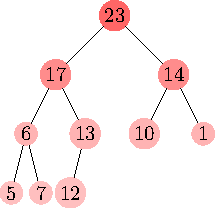
\includegraphics[scale=1.5]{img/6_1-6/6_1-6.pdf}
        \caption{Tas sous forme d'arbre du tableau $\langle 23, 17, 14, 6, 13, 10, 1, 5, 7, 12\rangle$}
          \label{fig:6.1-6}
        \end{figure}
    \end{ex}
  \descitem{6.1-7} \textit{Show that, with the array representation for storing an $n$-element heap, the leaves are the nodes indexed by $\lfloor n/2 \rfloor +1, \lfloor n/2\rfloor + 2, \ldots, n$.}
    \begin{ex}
      Une feuille n'a pas de fils, et comme les n\oe ux sont ins\'er\'es de fa\c{c}on contig\"ue, il suffit de trouver le premier    $k$ tel que $\textsc{Left}(k) =2k > n$. On a donc $n/2 < k$ et puis comme $k$ est un entier, il vaut $\lfloor n/2 \rfloor +1$.
    \end{ex}
\end{description}

\subsection{Maintaining the heap property}

\begin{description}
  \descitem{6.2-1} \textit{Using Figure 6.2 as a model, illustrate the operation of $\proc{Max-Heapify}(A,3)$ on the array $A = \langle 27, 17, 3, 16, 13, 10, 1, 5, 7, 12, 4, 8, 9, 0 \rangle$}
    \begin{ex}

      Regardons la figure (\ref{fig:Heapify}) qui illustre les op\'erations de $\proc{Max-Heapify}(A,3)$ : (\subref{fig:6_2-1_1}) La configuration initiale du tas, avec la valeur $A[3]$ au n\oe ud $i = 3$ viole la propri\'et\'e de \textit{max-heap} puisque'elle n'est pas sup\'erieur \`a celle des enfants. La propri\'et\'e de \textit{max-heap} est restaur\'ee pour le n\oe ud $3$ en (\subref{fig:6_2-1_2}) via \'echange de $A[3]$ avec $A[6]$, ce qui d\'etruit la propri\'et\'e de \textit{max-heap} pour le n\oe ud $6$. L'appel r\'ecursif $\proc{Max-Heapify}(A,6)$ prend maintenant $i=6$. Apr\`es  avoir \'echang\'e $A[6]$ avec $A[13]$, comme illustr\'e en (\subref{fig:6_2-1_3}), le n\oe ud $6$ est corrig\'e, et l'appel r\'ecursif $\proc{Max-Heapify}(A,13)$ n'engendre plus de modifications de la structure de donn\'ees.

      \begin{figure}[H]
        \centering
        \begin{subfigure}[t]{.45\textwidth}
          \centering
          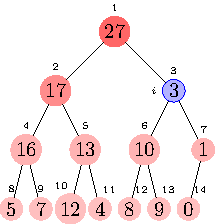
\includegraphics[scale=1.4]{img/6_2-1/6_2-1_1}
          \caption{}\label{fig:6_2-1_1}
        \end{subfigure}

        \begin{subfigure}[t]{.45\textwidth}
          \centering
          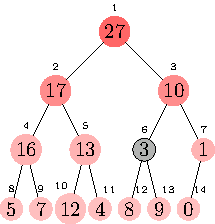
\includegraphics[scale=1.4]{img/6_2-1/6_2-1_2}
          \caption{}\label{fig:6_2-1_2}
        \end{subfigure}
        \begin{subfigure}[t]{.45\textwidth}
          \centering
          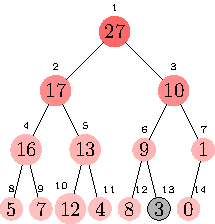
\includegraphics[scale=1.4]{img/6_2-1/6_2-1_3}
          \caption{}\label{fig:6_2-1_3}
        \end{subfigure}
        \caption{L'action $\proc{Max-Heapify}(A,3)$,o\`u $\attrib{A}{heap-size}= 14$.} 
        \label{fig:Heapify}
      \end{figure}
    \end{ex}
  \descitem{6.2-2} \textit{Starting with the procedure \proc{Max-Heapify}, write pseudocode for the procedure $\proc{Min-Heapify}(A,i)$ which performs the corresponding manipulation on a min-heap. How does the running time of \proc{Min-Heapify} compare to that of \proc{Max-Heapify} ?}
    \begin{ex}
      \begin{codebox}
        \Procname{\algo{Min-Heapify}$(A,i)$}
        \li $l = \proc{Left}(i)$
        \li $r = \proc{Right}(i)$
        \li \If $l \le \attrib{A}{heap-size}$ and $A[l] < A[i]$ \Do
        \li $\id{least} = l$        
        \li \Else $\id{least} = i$ \End
        \li \If $r \le \attrib{A}{heap-size}$ and $A[r] < A[least]$ \Do
        \li $\id{least} = r$  \End    
        \li \If $\id{least} \ne i$ \Do
        \li $\func{swap}(A,i,\id{least})$
        \li $\proc{Min-Heapify}(A,least)$
      \end{codebox}
      L'algorithme \'etant la m\^eme que celle du \proc{Max-Heapify} \`a quelques signes pr\`es, on est certain qu'ils ont la m\^eme complexit\'e en temps. D\'etaillons quand m\^eme la preuve du livre. 
      Le temps d'ex\'ecution de \proc{Min-Heapify} est le temps $\Theta(1)$ n\'ecessaire pour corriger les relations entre les \'el\'ements, plus le temps d'ex\'ecuter \proc{Min-Heapify} sur un sous-arbre enracin\'e sur l'un des enfants du n\oe ud $i$. 
      
      Majorons la taille du sous-arbre de gauche.  On sait que le pire des cas survient quand la derni\`ere rang\'ee de l'arbre est remplie \`a moiti\'e, alors on a la ratio suivant : 
      \[R_n = \frac{\textrm{taille de l'arbre enracin\'e sur le n\oe ud  } \proc{Left}(i)}{\textrm{taille de l'arbre enracin\'e sur le n\oe ud } i} = \frac{2^{n-1}-1}{2^n-2^{n-2}-1}.\]
      $R_n$ est croissante et admet une limite $R_n \underset{n \to +\infty}{\longrightarrow} 2/3$ qui est le major\'e de la taille du sous-arbre de gauche. Ainsi, on obtient l'in\'egalit\'e : \[T(n) \le T(2n/3) + \Theta(1).\]
      Puis on utilise le \textit{master theorem}. Dans notre cas $f(n) = \Theta(1)$ et $n^{\log_{3/2}1} = 1$. Le deuxi\`eme cas convient, on a bien $f(n) = \Theta(1)$, donc la solution est $T(n) = O(\lg n) = O(h)$ avec $h$ l'hauteur de l'arbre (d'apr\`es \descref{6.1-2}, $h = \lfloor \lg n \rfloor$). 
    \end{ex}
  \descitem{6.2-3} \textit{What is the effect of calling $\proc{Max-Heapify}(A,i)$ when the element $A[i]$ is larger than its children?}
    \begin{ex}
      L'algorithme effectue les comparaisons n\'ecessaires et s'arr\^ete en temps constant. Aucun \'echange a lieu car le n\oe ud et ses fils v\'erifient la propri\'et\'e d'un \textit{max-heap}.
    \end{ex}
  \descitem{6.2-4} \textit{What is the effect of calling $\proc{Max-Heapify}(A,i)$ for $i > \attrib{A}{heap-size}/2$?}
    \begin{ex}
      On a $\lfloor \attrib{A}{heap-size}/2 \rfloor + 1 \le i \le \attrib{A}{heap-size}$, d'apr\`es \descref{6.1-7}, tous les n\oe ud d'indice $i$ sont des feuilles. Donc l'algorithme s'arr\^ete en temps constant et aucun \'echange a lieu.
    \end{ex}
  \descitem{6.2-5} \textit{The code for \proc{Max-Heapify} is quite efficient in terms of constant factors, except
possibly for the recursive call in line 10, which might cause some compilers to
produce inefficient code. Write an efficient \proc{Max-Heapify} that uses an iterative
control construct (a loop) instead of recursion.}
    \begin{ex}
      \begin{codebox}
        \Procname{\algo{Iterative-Max-Heapify}$(A,i)$}
        \li \While $\proc{Left}(i) < \attrib{A}{heap-size}$ and $\proc{Right}(i) < \attrib{A}{heap-size}$ \Do
        \li $l = \proc{Left}(i)$
        \li $r = \proc{Right}(i)$
        \li \Comment Les lignes \ref{li:IMH-begin-compare}-\ref{li:IMH-end-compare} peuvent \^etre exprimer autrement
      \footnote{$\id{largest} = \func{index-of-max}(A[i], A[l], A[r])$.}
        \li \If  $A[l] > A[i]$ \Do           \label{li:IMH-begin-compare} 
        \li $\id{largest} = l$        
        \li \Else $\id{largest} = i$ \End
        \li \If  $A[r] > A[largest]$ \Do
        \li $\id{largest} = r$  \End         \label{li:IMH-end-compare}
        \li \If $\id{largest} \ne i$ \Do
        \li $\func{swap}(A,i,\id{largest})$ 
        \li $i = \id{largest}$
        \li \Else \Return \End
        \End 
      \end{codebox}
    \end{ex}
  \descitem{6.2-6} \textit{Show that the worst-case running time of \proc{Max-Heapify} on a heap of size $n$
is $\Omega(\lg n)$. (Hint: For a heap with $n$ nodes, give node values that cause \proc{Max-Heapify}
 to be called recursively at every node on a simple path from the root down to a leaf.)}
    \begin{ex}
      Le pire cas a lieu lorsqu'il existe un chemin tel que ses \'el\'ements sont tri\'es de mani\`ere croissante. Dans ce cas l\`a, il y a exactement $h = \lfloor \lg n\rfloor$ appels recursives de la fonction \proc{Max-Heapify}. D'o\`u la borne inf\'erieure $\Omega(\lg n)$.
    \end{ex} 
\end{description}

\subsection{Building a heap}

\begin{description}
    \descitem{6.3-1} \textit{Using Figure 6.3 as a model, illustrate the operation of \proc{Build-Max-Heap} on the
array $A = \langle 5, 3, 17, 10, 84, 19, 6, 22, 9 \rangle$.}
    \begin{ex}
	 Observons la figure (\ref{fig:Build-Max-Heap}) : (\subref{fig:6_3-1_1}) Un tableau de 9 \'el\'ements en entr\'ee, avec l'arbre binaire qu'il repr\'esente. La figure montre que l'indice de boucle $i$ pointe vers le n\oe ud 4 avant l'appel $\proc{Max-Heapify}(A,i)$. (\subref{fig:6_3-1_2}) La structure de donn\'ees r\'esultante. L'indicde de boucle $i$ de l'it\'eration suivante pointe vers le n\oe ud $3$. (\subref{fig:6_3-1_3})-(\subref{fig:6_3-1_4}) Les it\'erations suivantes de la boucle \textbf{for} de \proc{Build-Max-Heap}. \`A chaque fois qu'il y a appel de \proc{Max-Heapify} sur un n\oe ud, les deux sous-arbres de ce n\oe ud sont des \textit{max-heap}. (\subref{fig:6_3-1_5}) Le \textit{max-heap} apr\`es que \proc{Build-Max-Heap} a fini.
      \begin{figure}[H]
        \centering
        \begin{subfigure}[t]{.45\textwidth}
          \centering
          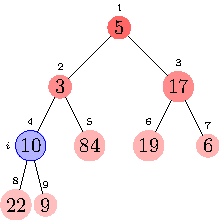
\includegraphics[scale=1.4]{img/6_3-1/6_3-1_1}
          \caption{}\label{fig:6_3-1_1}
        \end{subfigure}
        \begin{subfigure}[t]{.45\textwidth}
          \centering
          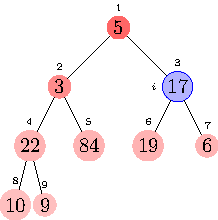
\includegraphics[scale=1.4]{img/6_3-1/6_3-1_2}
          \caption{}\label{fig:6_3-1_2}
        \end{subfigure}
        \begin{subfigure}[t]{.45\textwidth}
          \centering
          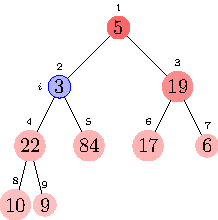
\includegraphics[scale=1.4]{img/6_3-1/6_3-1_3}
          \caption{}\label{fig:6_3-1_3}
        \end{subfigure}
        \begin{subfigure}[t]{.45\textwidth}
          \centering
          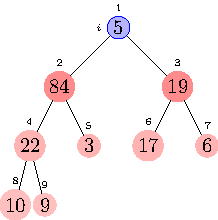
\includegraphics[scale=1.4]{img/6_3-1/6_3-1_4}
          \caption{}\label{fig:6_3-1_4}
        \end{subfigure}
        \begin{subfigure}[t]{.45\textwidth}
          \centering
          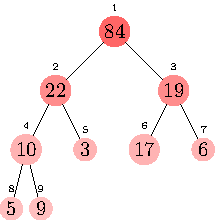
\includegraphics[scale=1.4]{img/6_3-1/6_3-1_5}
          \caption{}\label{fig:6_3-1_5}
        \end{subfigure}
        \caption{Le fonctionnement de $\proc{Build-Max-Heap}(A)$, o\`u $\attrib{A}{heap-size}= 9$.} 
        \label{fig:Build-Max-Heap}
      \end{figure}
    \end{ex}
    \descitem{6.3-2} \textit{Why do we want the loop index $i$ in line 2 of \proc{Build-Max-Heap} to decrease from
$\lfloor \attrib{A}{length}/2 \rfloor$ to $1$ rather than increase from $1$ to $\lfloor \attrib{A}{length}/2 \rfloor$ ?}
    \begin{ex}
	  L'hypoth\`ese de $\proc{Max-Heapify}(A,i)$ est que les sous-arbres $\proc{Left}(i)$ et $\proc{Right}(i)$ sont des \textit{max-heap}s. Si l'on commence par le n\oe ud $1$, alors il n'y a aucune garantie que les n\oe uds parcourus seront toujours des \textit{max-heap}s.
    \end{ex}
    \descitem{6.3-3} \textit{Show that there are at most $\lceil n/2^{h+1}\rceil$ nodes of height $h$ in any $n$-element heap.}
    \begin{ex} %TODO:relire et changer les notations
      Notons que les n\oe uds ayant une hauteur $j$ deviennent des feuilles apr\`es qu'on \^ote ceux qui ont comme hauteur $0, \ldots, j-1$. Sachant qu'un tas ayant $n$ \'el\'ements a exactement $n - \lfloor n/2 \rfloor = \lceil n/2 \rceil$ feuilles (d'apr\`es l'exercice \descref{6.1-7} et une identit\'e de partie enti\`ere du chapitre 3), on peut \'etablir deux suites r\'ecurrentes :
\[
\begin{matrix}
\left\{
	\begin{array}{ll}
	N_0 = n\\
	N_{i+1} = N_i - F_i
	\end{array}
\right.  &
\left\{
	\begin{array}{ll}
	F_0 = \lceil N_0/2 \rceil\\
	F_i = \lceil N_i/2 \rceil
	\end{array}
  \right. 
\end{matrix}
\]
o\`u $N_i$ d\'esigne le nombre de n\oe uds apr\`es avoir \^oter les n\oe uds de hauteur r\'espectives $0, \ldots, i-1$ et $F_i$ le nombre de feuilles de ce nouveau arbre.
\`A partir de ces relations, il en d\'ecoule que
\[ N_{i+1} = N_i - \lceil N_i/2 \rceil = \lfloor N_i/2 \rfloor \le N_i/2 \]
puis, par it\'eration, on a $N_i \le n/2^i$. On conclut que $F_i = \lceil N_i/2 \rceil \le \lceil n/2^{i+1} \rceil$.
    \end{ex}
\end{description}

\subsection{The heapsort algorithm}

\begin{description}
\descitem{6.4-1} \textit{Using Figure 6.4 as a model, illustrate the operation of \proc{Heapsort} on the array \\$A = \langle 5, 13, 2, 25, 7, 17, 20, 8, 4 \rangle$.}
    \begin{ex}
      Regardons la figure (\ref{fig:Heap-Sort}). (\subref{fig:6_4-1_1}) L'arbre binaire avant l'appel de  \proc{Build-Max-Heap}. (\subref{fig:6_4-1_2}) la structure de \textit{max-heap} juste apr\`es sa construction par \proc{Build-Max-Heap}. (\subref{fig:6_4-1_3})-(\subref{fig:6_4-1_10}) Le \textit{max-heap} juste apr\`es chaque appel de \proc{Max-Heapify}. La valeur de $i$ \`a ce moment est montr\'ee. Seul les n\oe uds rouges restent dans le tas.
      \begin{figure}[H]%TODO:rajouter le resulta dans une subfigure sous forme de tableau
        \centering
        \begin{subfigure}[t]{.30\textwidth}
          \centering
          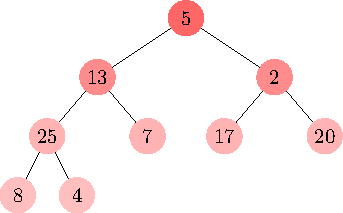
\includegraphics[scale=0.8]{img/6_4-1/6_4-1_1}
          \caption{}\label{fig:6_4-1_1}
        \end{subfigure}
        \begin{subfigure}[t]{.30\textwidth}
          \centering
          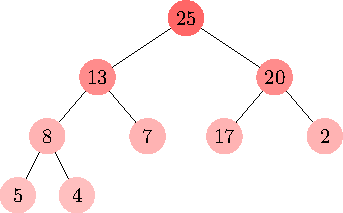
\includegraphics[scale=0.8]{img/6_4-1/6_4-1_2}
          \caption{}\label{fig:6_4-1_2}
        \end{subfigure}
        \begin{subfigure}[t]{.30\textwidth}
          \centering
          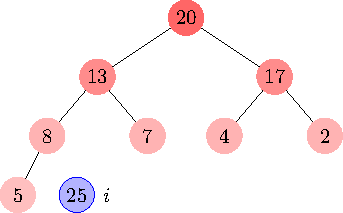
\includegraphics[scale=0.8]{img/6_4-1/6_4-1_3}
          \caption{}\label{fig:6_4-1_3}
        \end{subfigure}
        \begin{subfigure}[t]{.30\textwidth}
          \centering
          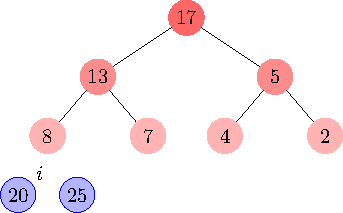
\includegraphics[scale=0.8]{img/6_4-1/6_4-1_4}
          \caption{}\label{fig:6_4-1_4}
        \end{subfigure}
        \begin{subfigure}[t]{.30\textwidth}
          \centering
          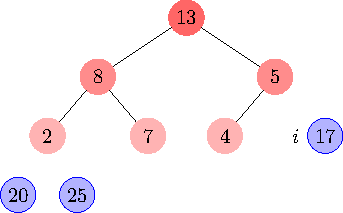
\includegraphics[scale=0.8]{img/6_4-1/6_4-1_5}
          \caption{}\label{fig:6_4-1_5}
        \end{subfigure}
        \begin{subfigure}[t]{.30\textwidth}
          \centering
          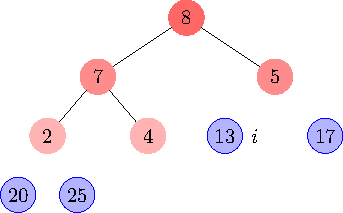
\includegraphics[scale=0.8]{img/6_4-1/6_4-1_6}
          \caption{}\label{fig:6_4-1_6}
        \end{subfigure}
        \begin{subfigure}[t]{.30\textwidth}
          \centering
          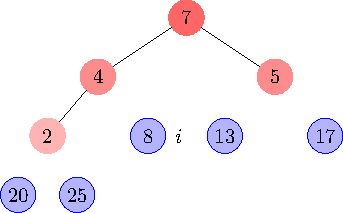
\includegraphics[scale=0.8]{img/6_4-1/6_4-1_7}
          \caption{}\label{fig:6_4-1_7}
        \end{subfigure}
        \begin{subfigure}[t]{.30\textwidth}
          \centering
          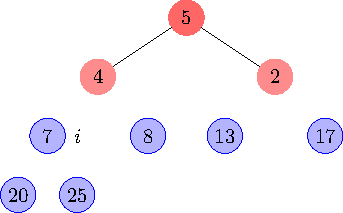
\includegraphics[scale=0.8]{img/6_4-1/6_4-1_8}
          \caption{}\label{fig:6_4-1_8}
        \end{subfigure}
        \begin{subfigure}[t]{.30\textwidth}
          \centering
          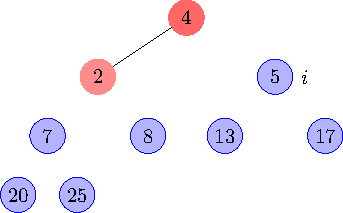
\includegraphics[scale=0.8]{img/6_4-1/6_4-1_9}
          \caption{}\label{fig:6_4-1_9}
        \end{subfigure}
        \begin{subfigure}[t]{.30\textwidth}
          \centering
          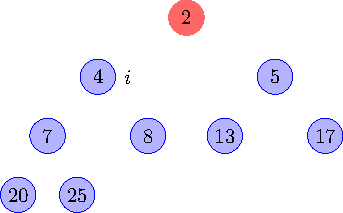
\includegraphics[scale=0.8]{img/6_4-1/6_4-1_10}
          \caption{}\label{fig:6_4-1_10}
        \end{subfigure}
        \caption{Le fonctionnement du $\proc{Heap-Sort}(A)$ sur $A = \langle 5, 13, 2, 25, 7, 17, 20, 8, 4 \rangle$.} 
        \label{fig:Heap-Sort}
      \end{figure}
    \end{ex}
\descitem{6.4-2} {\itshape Argue the correctness of \proc{Heap-Sort} using the following loop invariant:

  At the start of each iteration of the \textbf{for} loop of lines 2–5, the subarray
$A[1 \twodots i]$ is a max-heap containing the $i$ smallest elements of $A[1 \twodots n]$, and
the subarray $A[i+1 \twodots n]$ contains the $n-i$ largest elements of $A[1 \twodots n]$,
sorted.}
    \begin{ex}
      \begin{description}
        \item[Initialisation :] Avant la premi\`ere it\'eration de la boucle, $i=n$. De plus, par construction de \proc{Build-Max-Heap}, $A[i\twodots n]$ est un \textit{max-heap}. Il contient le $n$-i\`eme plus petit (autrement dit le plus grand) \'el\'ement qui n'est rien d'autre que la racine du tas. Le sous-tableau $A[i+1\twodots n]$ est vide, donc ne contient aucun \'el\'ement tri\'e.
        \item[Maintenance :] Supposons, au d\'ebut de l'it\'eration \`a laquelle $i=k$, que le tableau $A[1\twodots i]$ est un \textit{max-heap} contenant le $i$-i\`eme plus petit \'el\'ement et que le tableau $A[i+1\twodots n]$ contient les $n-i$ plus grands \'el\'ements de $A[1\twodots n]$ tri\'es d'ordre croissant. $A[1\twodots i]$ \'etant un \textit{max-heap}, $A[1]$ est donc le plus grand \'el\'ement. En l'\'echangeant avec $A[i]$, $A[i\twodots n]$ contient les $n-i+1$ plus grands \'el\'ements de $A[1\twodots n]$. En outre, en cas d'existence, $\proc{Left}(1)$ et $\proc{Right}(1)$ sont des \textit{max-heap}s, ainsi en appliquant \proc{Max-Heapify} au n\oe ud $1$, il est garantie que $A[1\twodots i-1]$ est un \textit{max-heap}. 
        \item[Terminaison :] Apr\`es l'it\'eration $i=2$, $A[1]$ est le plus petit \'el\'ement de $A[1\twodots n]$ et $A[2\twodots n]$ est tri\'e de mani\`ere croissante, donc $A[1 \twodots n]$ est tri\'e.
      \end{description}
    \end{ex}
\descitem{6.4-3} \textit{What is the running time of \proc{Heap-sort} on an array $A$ of length n that is already
sorted in increasing order? What about decreasing order?}
    \begin{exrev}
      
    \end{exrev}
\descitem{6.4-4} \textit{Show that the worst-case running time of \proc{Heapsort} is $\Omega (n \lg n)$.}
    \begin{exrev}
      
    \end{exrev}
  \item[6.4-5 $\star$]  \textit{Show that when all elements are distinct, the best-case running time of \proc{Heap-Sort}
is $\Omega(n \lg n)$.}
    \begin{exrev}
      
    \end{exrev}
\end{description}

\subsection{Priority queues}

\begin{description}
    \descitem{6.5-1} \textit{Illustrate the operation of \proc{Heap-Extract-Max} on the heap \\$A = \langle 15, 13, 9, 5, 12, 8, 7, 4, 0, 6, 2,1 \rangle$.}
        \begin{ex}
          Consid\'erons la figure (\ref{fig:Heap-Extract-Max}). (\subref{fig:6_5-1_1}) Le tas $A$ avant l'extraction. (\subref{fig:6_5-1_2}) L'extraction du plus grand \'el\'ement $A[1]=15$. (\subref{fig:6_5-1_3})-(\subref{fig:6_5-1_5}) L'application de $\proc{Max-Heapify}(A,1)$. (\subref{fig:6_5-1_6}) On obtient \`a nouveau un \textit{max-heap} et on retourne \id{max}.
      \begin{figure}[H]
        \centering
        \begin{subfigure}[t]{.40\textwidth}
          \centering
          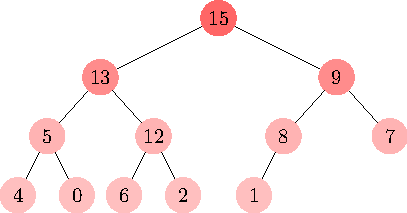
\includegraphics[scale=0.8]{img/6_5-1/6_5-1_1}
          \caption{}\label{fig:6_5-1_1}
        \end{subfigure}
        \begin{subfigure}[t]{.40\textwidth}
          \centering
          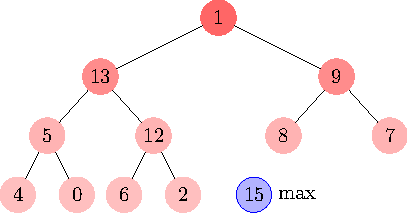
\includegraphics[scale=0.8]{img/6_5-1/6_5-1_2}
          \caption{}\label{fig:6_5-1_2}
        \end{subfigure}
        \begin{subfigure}[t]{.40\textwidth}
          \centering
          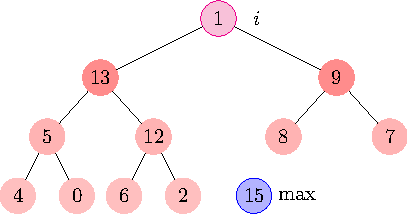
\includegraphics[scale=0.8]{img/6_5-1/6_5-1_3}
          \caption{}\label{fig:6_5-1_3}
        \end{subfigure}
        \begin{subfigure}[t]{.40\textwidth}
          \centering
          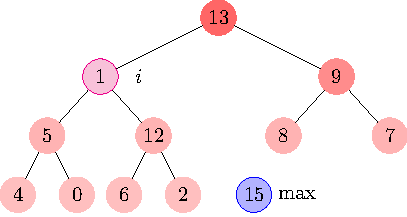
\includegraphics[scale=0.8]{img/6_5-1/6_5-1_4}
          \caption{}\label{fig:6_5-1_4}
        \end{subfigure}
        \begin{subfigure}[t]{.40\textwidth}
          \centering
          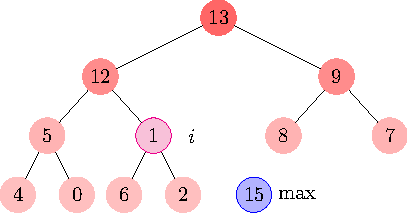
\includegraphics[scale=0.8]{img/6_5-1/6_5-1_5}
          \caption{}\label{fig:6_5-1_5}
        \end{subfigure}
        \begin{subfigure}[t]{.40\textwidth}
          \centering
          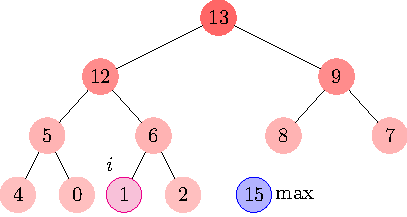
\includegraphics[scale=0.8]{img/6_5-1/6_5-1_6}
          \caption{}\label{fig:6_5-1_6}
        \end{subfigure}
        \caption{\centering Le fonctionnement de $\proc{Heap-Extract-Max}(A)$\\ sur $A = \langle 15, 13, 9, 5, 12, 8, 7, 4, 0, 6, 2,1 \rangle$.} 
        \label{fig:Heap-Extract-Max}
      \end{figure}
        \end{ex}
    \descitem{6.5-2} \textit{Illustrate the operation of \proc{Max-Heap-Insert} on the heap \\$A = \langle 15, 13, 9, 5, 12, 8, 7, 4, 0, 6, 2,1 \rangle$.}
        \begin{exrev}
          
        \end{exrev}
    \descitem{6.5-3} \textit{Write pseudocode for the procedures \proc{Heap-Minimum}, \proc{Heap-Extract-Min}, \proc{Heap-Decrease-Key}, and \proc{Min-Heap-Insert} that implement a min-priority queue with a min-heap.}
        \begin{exrev}
          
        \end{exrev}
    \descitem{6.5-4} \textit{Why do we bother setting the key of the inserted node to $-\infty$ in line 2 of \proc{Max-Heap-Insert} when the next thing we do is increase its key to the desired value ?}
        \begin{exrev}
          
        \end{exrev}
    \descitem{6.5-5} {\itshape Argue the correctness of \proc{Heap-Increase-Key} using the following loop invariant :

At the start of each iteration of the \textbf{while} loop of lines 4–6, the subarray
$A[1 \twodots \attrib{A}{heap-size}]$ satisfies the max-heap property, except that there may
be one violation: $A[i]$ may be larger than $A[\proc{Parent}(i)]$.

You may assume that the subarray $A[1 \twodots \attrib{A}{heap-size}]$ satisfies the max-heap property at the time \proc{Heap-Increase-Key} is called.
}

        \begin{exrev}
          
        \end{exrev}
    \descitem{6.5-6} \textit{Each exchange operation on line 5 of \proc{Heap-Increase-Key} typically requires
three assignments. Show how to use the idea of the inner loop of \proc{Insertion-Sort} to reduce the three assignments down to just one assignment.}
        \begin{exrev}
          
        \end{exrev}
    \descitem{6.5-7} \textit{Show how to implement a first-in, first-out queue with a priority queue. Show
how to implement a stack with a priority queue. (Queues and stacks are defined in
Section 10.1.)}
        \begin{exrev}
          
        \end{exrev}
    \descitem{6.5-8} \textit{The operation $\proc{Heap-Delete}(A,i)$ deletes the item in node $i$ from heap $A$. Give
an implementation of \proc{Heap-Delete} that runs in $O (\lg n)$ time for an $n$-element
max-heap.}
        \begin{exrev}
          
        \end{exrev}
    \descitem{6.5-9} \textit{Give an $O(n \lg k)$-time algorithm to merge $k$ sorted lists into one sorted list,
where $n$ is the total number of elements in all the input lists. (Hint: Use a min-heap for $k$-way merging.)}
        \begin{exrev}
          
        \end{exrev}
\end{description}


\section{Quicksort}
\subsection{Description of quicksort}
\subsection{Performance of quicksort}
\subsection{A randomized version of quicksort}
\subsection{Analysis of quicksort}

\section{Sorting in Linear Time}
\subsection{Lower bounds for sorting}
\subsection{Counting sort}
\subsection{Radix sort}
\subsection{Bucket sort}

\section{Medians and Order Statistics}

\part{Data Structures}
\section{Elementary Data Structures}
\subsection{Stacks and queues}
\label{sub:stacks_and_queues}



\begin{description}

\descitem{10.1-1} \textit{Using Figure 10.1 as a model, illustrate the result of each operation in the sequence $\proc{Push}(S,4)$, $\proc{Push}(S,1)$,$\proc{Push}(S,3)$, $\proc{Pop}(S)$, $\proc{Push}(S,8)$, and $\proc{Pop}(S)$  on an initially empty stack $S$ stored in array $S[1 \twodots6]$.}
\begin{ex}
    \begin{figure}[H]
      \centering
      \begin{subfigure}[t]{.45\textwidth}
        \centering
        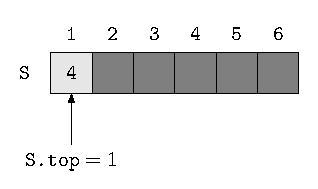
\includegraphics[scale=1]{img/10_1-1/10_1-1_1.pdf}
        \caption{$\proc{Push}(S,4)$}\label{fig:10_1-1_1}
      \end{subfigure}
      \begin{subfigure}[t]{.45\textwidth}
        \centering
        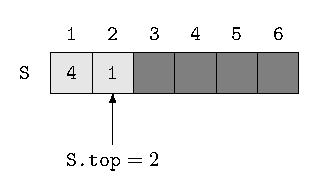
\includegraphics[scale=1]{img/10_1-1/10_1-1_2.pdf}
        \caption{$\proc{Push}(S,1)$}\label{fig:10_1-1_2}
      \end{subfigure}
      \begin{subfigure}[t]{.45\textwidth}
        \centering
        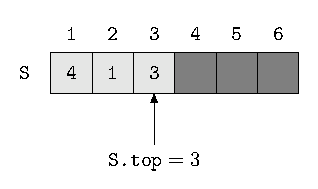
\includegraphics[scale=1]{img/10_1-1/10_1-1_3.pdf}
        \caption{$\proc{Push}(S,3)$}\label{fig:10_1-1_3}
      \end{subfigure}
      \begin{subfigure}[t]{.45\textwidth}
        \centering
        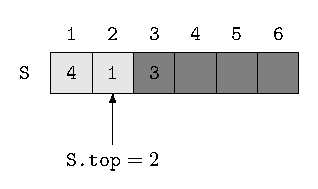
\includegraphics[scale=1]{img/10_1-1/10_1-1_4.pdf}
        \caption{$\proc{Pop}(S)$}\label{fig:10_1-1_4}
      \end{subfigure}
      \begin{subfigure}[t]{.45\textwidth}
        \centering
        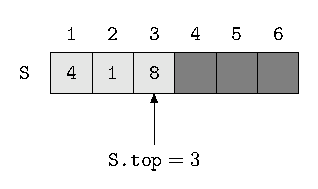
\includegraphics[scale=1]{img/10_1-1/10_1-1_5.pdf}
        \caption{$\proc{Push}(S,8)$}\label{fig:10_1-1_5}
      \end{subfigure}
      \begin{subfigure}[t]{.45\textwidth}
        \centering
        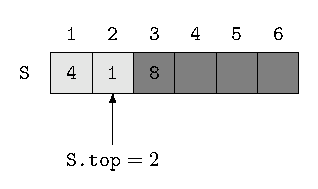
\includegraphics[scale=1]{img/10_1-1/10_1-1_6.pdf}
        \caption{$\proc{Pop}(S)$}\label{fig:10_1-1_6}
      \end{subfigure}
      \caption{Séquence d'opérations sur une pile vide de taille 6.} 
      \label{fig:stack-seq} 
    \end{figure}
\end{ex}
\descitem{10.1-2} \textit{Explain how to implement two stacks in one array $A[1\twodots n]$ in such a way that neither stack overflows unless the total number of elements in both stacks together is $n$. The \proc{Push} and \proc{Pop} operations should run in $O(1)$ time.}
\begin{ex}
  Il suffit d'initialiser les piles aux extrémités du tableau, \textit{i.e.} $S_1.\textrm{top} = 1$ et $S_2.\textrm{top} = n$. La pile $S_1$ fonctionne comme montré à la fig. \ref{fig:stack-seq} et la pile $S_2$ décrémente l'indice du sommet lors d'un \proc{Push} et l'incrémente lors d'un \proc{Pop}. Lorsque le nombre total des éléments des deux piles est égale à $n$, il y a overflow si on empile un élément dans une des piles. Les primitives \proc{Push} et \proc{Pop} sont bien de $O(1)$.
  %TODO:Tikz:illustration ?
\end{ex}
\descitem{10.1-3} \textit{Using Figure 10.2 as a model,  illustrate the result of each operation in the sequence $\proc{Enqueue}(Q, 4)$, $\proc{Enqueue}(Q, 1)$, $\proc{Enqueue}(Q, 3)$, $\proc{Dequeue}(Q)$,  $\proc{Enqueue}(Q, 8)$,  and $\proc{Dequeue}(Q)$ on an initially empty queue $Q$ stored in array $Q[1 \twodots 6]$.}
\begin{ex}
  
    \begin{figure}[H]
      \centering
      \begin{subfigure}[t]{.45\textwidth}
        \centering
        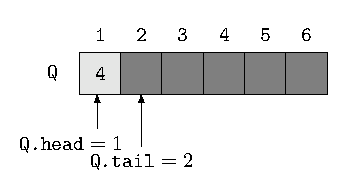
\includegraphics[scale=1]{img/10_1-3/10_1-3_1.pdf}
        \caption{$\proc{Enqueue}(Q,4)$}\label{fig:10_1-3_1}
      \end{subfigure}
      \begin{subfigure}[t]{.45\textwidth}
        \centering
        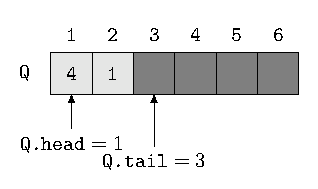
\includegraphics[scale=1]{img/10_1-3/10_1-3_2.pdf}
        \caption{$\proc{Enqueue}(Q,1)$}\label{fig:10_1-3_2}
      \end{subfigure}
      \begin{subfigure}[t]{.45\textwidth}
        \centering
        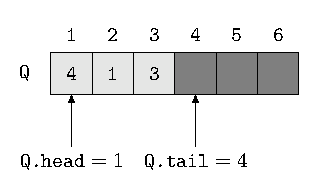
\includegraphics[scale=1]{img/10_1-3/10_1-3_3.pdf}
        \caption{$\proc{Enqueue}(Q,3)$}\label{fig:10_1-3_3}
      \end{subfigure}
      \begin{subfigure}[t]{.45\textwidth}
        \centering
        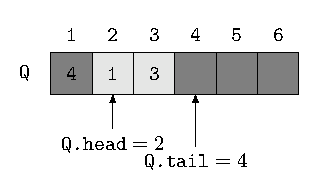
\includegraphics[scale=1]{img/10_1-3/10_1-3_4.pdf}
        \caption{$\proc{Dequeue}(Q)$}\label{fig:10_1-3_4}
      \end{subfigure}
      \begin{subfigure}[t]{.45\textwidth}
        \centering
        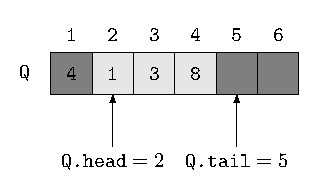
\includegraphics[scale=1]{img/10_1-3/10_1-3_5.pdf}
        \caption{$\proc{Enqueue}(Q,8)$}\label{fig:10_1-3_5}
      \end{subfigure}
      \begin{subfigure}[t]{.45\textwidth}
        \centering
        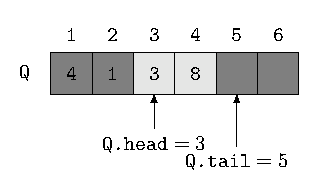
\includegraphics[scale=1]{img/10_1-3/10_1-3_6.pdf}
        \caption{$\proc{Dequeue}(Q)$}\label{fig:10_1-3_6}
      \end{subfigure}
      \caption{Séquence d'opérations sur une file vide de taille 6.} 
      \label{fig:queue-seq} 
    \end{figure}
\end{ex}
\descitem{10.1-4} \textit{Rewrite \proc{Enqueue} and \proc{Dequeue} to detect underflow and overflow of a queue.}
\begin{ex}
  La description donnée ne permet pas de déterminer si une file est vide ou pleine. Supposons, par commodité, que la file est implémenté sur le tableau $Q[0\twodots n-1]$ (cette hypothèse est pratique pour l'arithmétique modulaire). Il existe plusieurs méthodes possibles pour contourner ce problème, on en présente ici trois :
  \begin{enumerate}[label=\circled{\arabic*}]
    \item Ajouter en attribue de la file un état \textit{isempty} qui vaut \const{true} si la file est vide et \const{false} inversement. La file est pleine lorsque $\attrib{Q}{head} = \attrib{Q}{tail}$ et $\attrib{Q}{isempty} = \const{false}$.

\begin{codebox}
\Procname{\textbf{Algorithme}\quad\textsc{Enqueue-1}$(\id{Q}, \id{e})$}
    \li \If $\attrib{Q}{head}\isequal\attrib{Q}{tail} \And \attrib{Q}{isempty} \isequal \const{false}$ \Then
        \li \Error "The queue is full : failed to enqueue." \End
    \li  $Q[\attrib{Q}{tail}] \gets e$ 
    \li $\attrib{Q}{tail} = (\attrib{Q}{tail}+1)\bmod \attrib{Q}{length}$
    \li \If $\attrib{Q}{isempty} \isequal \const{true}$ \Then
      \li $\attrib{Q}{isempty} \gets \const{false}$ \End
\end{codebox}
\begin{codebox}
\Procname{\textbf{Algorithme}\quad\textsc{Dequeue-1}$(\id{Q})$}
    \li \If $\attrib{Q}{isempty}$ \Then
        \li \Error "The queue is empty: failed to dequeue." \End
    \li  $\id{e} \gets Q[\attrib{Q}{head}]$ 
    \li $\attrib{Q}{head} = (\attrib{Q}{head}+1)\bmod \attrib{Q}{length}$
    \li \If $\attrib{Q}{head} \isequal \attrib{Q}{tail}$ \Then
      \li $\attrib{Q}{isempty} \gets \const{true}$ \End
    \li \Return \id{e}
\end{codebox}
    \item Faire pointer $\attrib{Q}{head}$ vers \const{Nil} si la file est vide. La file est pleine lorsque $\attrib{Q}{head} = \attrib{Q}{tail}$.
\begin{codebox}
\Procname{\textbf{Algorithme}\quad\textsc{Enqueue-2}$(\id{Q}, \id{e})$}
    \li \If $\attrib{Q}{head}\isequal\attrib{Q}{tail}$ \Then
        \li \Error "The queue is full : failed to enqueue." \End
    \li  $Q[\attrib{Q}{tail}] \gets e$ 
    \li $\attrib{Q}{tail} = (\attrib{Q}{tail}+1)\bmod \attrib{Q}{length}$
\end{codebox}
\begin{codebox}
\Procname{\textbf{Algorithme}\quad\textsc{Dequeue-2}$(\id{Q})$}
    \li \If $\attrib{Q}{head}\isequal\const{Nil}$ \Then
        \li \Error "The queue is empty: failed to dequeue." \End
    \li  $\id{e} \gets Q[\attrib{Q}{head}]$ 
    \li $\attrib{Q}{head} = (\attrib{Q}{head}+1)\bmod \attrib{Q}{length}$
    \li \If $\attrib{Q}{head} \isequal \attrib{Q}{tail}$ \Then
      \li $\attrib{Q}{head} \gets \const{Nil}$ \End
    \li \Return \id{e}
\end{codebox}
    \item \footnote{L'implémentation des algorithmes suivantes se trouve dans le dossier \pathx{src/CH10_Elementary_Data_Structures/Queue/}.}
    À la place de $\attrib{Q}{head}$ et $\attrib{Q}{tail}$, on utilise $\attrib{Q}{front}$ et $\attrib{Q}{count}$. $\attrib{Q}{front}$ joue le même rôle que $\attrib{Q}{tail}$. L'emplacement de $\attrib{Q}{head}$ peut se déduire à partir de l'identité :
        \[\attrib{Q}{head} + \attrib{Q}{count}\equiv \attrib{Q}{tail}\pmod{\attrib{Q}{length}}.\]
    Dans ce cas, la file est vide si $\attrib{Q}{count} = 0$ et pleine si $\attrib{Q}{count} = \attrib{Q}{length}$. 
\begin{codebox}
\Procname{\algo{Enqueue-With-Counter}$(\id{Q}, \id{e})$}
    \li \If $\attrib{Q}{count}\isequal\attrib{Q}{length}$ \Then
        \li \Error "The queue is full : failed to enqueue." \End
    \li  $Q[\attrib{Q}{front}] \gets e$ 
    \li $\attrib{Q}{count} = \attrib{Q}{count}+1$
    \li $\attrib{Q}{front} = (\attrib{Q}{front}+1)\bmod \attrib{Q}{length}$
\end{codebox}
\begin{codebox}
\Procname{\algo{Dequeue-With-Counter}$(\id{Q})$}
    \li \If $\attrib{Q}{count}\isequal0$ \Then
        \li \Error "The queue is empty: failed to dequeue." \End
    \li  $\id{e} \gets Q[(\attrib{Q}{front} - \attrib{Q}{count} + \attrib{Q}{length}) \bmod \attrib{Q}{length}]$ \label{li:dequeue-counter-tail}
    \li  $\attrib{Q}{count} = \attrib{Q}{count}-1$
    \li \Return \id{e}
\end{codebox}
\textit{N.B.} À la ligne \ref{li:dequeue-counter-tail} de l'algorithme \textsc{Dequeue-With-Counter}, on ajoute $\attrib{Q}{length}$ pour assurer que l'indice soit positive. 
  \end{enumerate} 
\end{ex}
\descitem{10.1-5} \textit{Whereas a stack allows insertion and deletion of elements at only one end, and a queue allows insertion at one end and deletion at the other end, a \textbf{deque} (double-ended queue) allows insertion and deletion at both ends. Write four $O(1)$-time procedures to insert elements into and delete elements from both ends of a deque implemented by an array.}
\begin{ex}
   On reprend les algorithmes \textsc{Enqueue-With-Counter} et \textsc{Dequeue-With-Counter} et les attribues définies. Les algorithmes suivantes complètent une file à une \textit{deque}.\footnote{L'implémentation des algorithmes suivantes se trouve dans le dossier \pathx{src/CH10_Elementary_Data_Structures/Deque/}.}
\begin{codebox}
\Procname{\algo{Enqueue-At-Other-End}$(\id{Q}, \id{e})$}
    \li \If $\attrib{Q}{count}\isequal\attrib{Q}{length}$ \Then
        \li \Error "The queue is full : failed to enqueue." \End
    \li  $Q[(\attrib{Q}{front} - (\attrib{Q}{count} + 1) + \attrib{Q}{length}) \bmod \attrib{Q}{length}] \gets e$ 
    \li $\attrib{Q}{count} = \attrib{Q}{count}+1$
\end{codebox}
\begin{codebox}
\Procname{\algo{Dequeue-At-Other-End}$(\id{Q})$}
    \li \If $\attrib{Q}{count}\isequal0$ \Then
        \li \Error "The queue is empty: failed to dequeue." \End
    \li  $\attrib{Q}{front} \gets (\attrib{Q}{front} -1 + \attrib{Q}{length}) \bmod \attrib{Q}{length}$
    \li  $\id{e} \gets Q[\attrib{Q}{front}]$ 
    \li  $\attrib{Q}{count} = \attrib{Q}{count}-1$
    \li \Return \id{e}
\end{codebox}
\end{ex}
\descitem{10.1-6} \textit{Show how to implement a queue using two stacks. Analyse the running time of the queue operations.}
\descitem{10.1-7} \textit{Show how to implement a stack using two queues. Analyse the running time of the queue operations.}


\end{description}

\subsection{Linked lists}
\label{sub:linked_lists}



\section{Hash Tables}

\section{Binary Search Trees}

\section{Red-Black Trees}

\section{Augmenting Data Structures}

\section{Dynamic Programming}

\section{Greedy Algorithms}

\section{Amortized Analysis}

\part{Advanced Data Structures}
\section{B-Trees}

\section{Fibonacci Heaps}

\section{van Emde Boas Trees}

\section{Data Structures for Disjoint Sets}

\clearpage
\part{Graph Algorithms}
\section{Elementary Graph Algorithms}

\subsection{Representations of graphs}

\begin{description}

\descitem{22.1-1} \textit{Given an adjacency-list representation of a directed graph, how long does it take to compute the out-degree of every vertex? How long does it take to compute the in-degrees?}    

\begin{ex}
Soient $G = (V,E)$ un graphe non-orienté, $v \in V$ un de ses sommets et $\attrib{G}{Adj}$ sa représentation en liste adjacente. On peut calculer le degré sortant de $v$ en calculant simplement la longueur de $\attrib{G}{Adj}[v]$. Ainsi, le calcul de degré sortant de tous les sommets se fait en $\Theta(V + E)$.

Pour calculer le degré entrant de $v$ on doit parcourir $\attrib{G}{Adj}$ entièrement. De cette manière, il nous faudra $\Theta(VE)$ en temps. On peut aussi implémenter une liste de taille $|V|$, indexé par ses sommets dans lequel chaque élément est initialisé par 0. Dans ce cas là, il suffit de parcourir $\attrib{G}{Adj}$ une fois en comptant chaque occurrence des sommets. Cette méthode a $\Theta(V + E)$ en complexité de temps et $\Theta(V)$ en espace.
\end{ex}


\descitem{22.1-2} \textit{Give an adjacency-list representation for a complete binary tree on $7$ vertices. Give an equivalent adjacency-matrix representation. Assume that vertices are numbered from $1$ to $7$ as in a binary heap.}    

%TODO:Horizontally centering subfigure
\begin{ex}
\begin{figure}[H]
\begin{subfigure}{0.45\textwidth}
\begin{table}[H]
\centering
\begin{tabular}{lll}
1: & 2 & 3 \\
2: & 4 & 5 \\
3: & 6 & 7 \\
4: & 2 &   \\
5: & 2 &   \\
6: & 3 &   \\
7: & 3 &  
\end{tabular}
\end{table}
\caption{Liste adjacente}
\end{subfigure}
\begin{subfigure}{0.45\textwidth}
\begin{center}
$$
\begin{pmatrix}
  0 & 1 & 1 & 0 & 0 & 0 & 0\\
  0 & 0 & 0 & 1 & 1 & 0 & 0\\
  0 & 0 & 0 & 0 & 0 & 1 & 1\\
  0 & 1 & 0 & 0 & 0 & 0 & 0\\
  0 & 1 & 0 & 0 & 0 & 0 & 0\\
  0 & 0 & 1 & 0 & 0 & 0 & 0\\
  0 & 0 & 1 & 0 & 0 & 0 & 0\\
\end{pmatrix}
$$
\end{center}
\caption{Matrice adjacente}
\end{subfigure}
\caption{Représentation de l'arbre complet de 7 sommets en liste adjacente et matrice adjacente}
\end{figure}
\end{ex}
\descitem{22.1-3} \textit{The \textbf{transpose} of a directed graph $G = (V, E)$ is the graph $G^T = (V, E^T)$, where $E^T = \{(v,u) \in V \times V : (u,v) \in E \}$. Thus, $G^T$ is $G$ with all its edges reversed.  Describe efficient algorithms for computing $G^T$ from $G$, for both the adjacency-list and adjacency-matrix representations of $G$. Analyze the running times of your algorithms.}    
\begin{ex}
Pour transposer une liste adjacente, il est nécessaire de la parcourir entièrement, donc la complexité est de $\Theta(V + E)$.
\begin{codebox}
\Procname{\algo{Transpose-Adj-List}$(\id{Adj})$}
    \li Create a new adjacency-list \id{newAdj}
    \li \For each linked-list $i$ of \id{Adj}\Do
    \li \For each element $j$ of \id{Adj}[i] \Do 
    \li $\attrib{newAdj[j]}{append(i)}$ \End \End
\end{codebox}
Quant à une matrice adjacente, il suffit de parcourir les éléments  supérieurs et les échanger à leur élément symétrique. De cette manière, il y a au total $\frac{n(n-1)}{2}$ d'échanges, d'où la complexité $\Theta(V^2)$.
\begin{codebox}
\Procname{\algo{Transpose-Adj-Matrix}$(M)$}
    \li \For $i \gets 1$ \To $\attrib{M}{size}$ \Do
    \li \For $j \gets i+1$ \To $\attrib{M}{size}$ \Do
    \li $\func{swap}(M[i,j],M[j,i])$ \End \End
\end{codebox}
\end{ex}
%TODO:english quote
\descitem{22.1-4} \textit{Given an adjacency-list representation of a multigraph $G = (V, E)$, describe an $O(V + E)$-time algorithm to compute the adjacency-list representation of the \foreignquote{english}{equivalent} undirected graph $G' = (V,E')$, where $E'$ consists of the edges in $E$ with all multiple edges between two vertices replaced by a single edge and with all self-loops removed.}    
\begin{ex}
\begin{codebox}
\Procname{\algo{Multigraph-To-Undigraph}$(\id{Adj})$}
    \li Create an array $A$ having length $|V|$ 
    \li \For each linked-list \id{Adj}[i]\Do
    \li $\func{init}(A)$ \Comment initialize all element to \const{false}
    \li \For each element $j$ of \id{Adj}[i] \Do 
    \li $e = \id{Adj[i][j]}$
    \li \If $e == i$ \Comment remove loop \Then 
    \li \attrib{Adj[i]}{remove(j)} 
    \li \Else 
    \li \If $A[e] == \const{true}$ \Comment remove multiple edge \Then
    \li \attrib{Adj[i]}{remove(j)} 
    \li \Else 
    \li $A[e] \gets \const{true}$\End
    \End \End
\end{codebox}
\end{ex}
\descitem{22.1-5} \textit{The \textbf{square} of a directed graph $G = (V, E)$ is the graph $G^2 = (V,E^2)$ such that $(u,v) \in E^2$   if and only if $G$ contains a path with at most two edges between $u$ and $v$. Describe efficient algorithms for computing $G^2$ from $G$ for both the adjacency-list and adjacency-matrix representations of $G$. Analyze the running times of your algorithms.}    
\begin{ex}
Dans le cas de matrice adjacente, on peut savoir l'existence d'une arrête en temps constant. Pour vérifier qu'il existe une arrête $(u,w) \in G^2$, on cherche toute paire d'arrête $(u,v)$ avec $v$ le sommet intermédiaire, puis en cas d'existence de $(u,v_0) \in G$, on cherche toute paire d'arrête $(v_0,w) \in G$. D'une telle manière, l'algorithme prend $\Theta(E^3)$.
\begin{codebox}
\Procname{\algo{Square-of-Adj-Matrix}$(M)$}
\li Create a matrix $M_2$ which have the same dimension of $M$
\li \For each vertex $i$ in $M$ \Do
  \li \For each vertex $j$ in $M[i]$ \Do
    \li \If $M[i][j]==1$ \Then
      \li \For each element $k$ in $M[j]$ \Do
        \li \If $M[i][k] == 1$ \Then
          \li $M_2[i][k] \gets 1$ 
        \End
        \li $M_2[i][k] \gets 1$ 
      \End 
    \End 
  \End
\End
\end{codebox}
%TODO:add explanation
\begin{codebox}
\Procname{\algo{Square-of-Adj-List}$(\id{Adj})$}
\li Create a new adjacency-list \id{newAdj}
\li \For each linked-list $i$ of $\id{Adj}$ \Do 
    \li \For each element $j$ of $\id{Adj}[i]$ \Do
        \li $\attrib{newAdj[i]}{append}(j)$ \Comment Add 1-length path
        \li \For each element $k$ of $\id{Adj}[j]$ \Do
            \li $\attrib{newAdj[i]}{append}(k)$ \Comment Add 2-length path
        \End
    \End
\end{codebox}
\end{ex}
\descitem{22.1-6} \textit{Most graph algorithms that take an adjacency-matrix representation as input require time $\Omega(V^2)$, but there are some exceptions. Show how to determine whether a directed graph $G$ contains a \textbf{universal sink} -- a vertex with in-degree $|V| - 1$ and out-degree $0$ -- in time $O(V)$, given an adjacency matrix for $G$.}    

\begin{exrev}
On cherche, dans la matrice adjacente, une colonne qui contient $|V|-1|$ 1. De cette manière, il suffit de parcourir qu'une fois le graphe entier, d'où la complexité $O(V)$.

%TODO:write the algo
\begin{codebox}
\Procname{\algo{Square-of-Adj-List}$(\id{M})$}
\li \For each vertex in 
\end{codebox}
\end{exrev}
%TODO:refer TD
\descitem{22.1-7} \textit{The \textbf{incidence matrix} of a directed graph $G = (V,E)$ with no self-loops is a $|V| \times |E|$ matrix $B = b_{ij}$ such that}
\[
    b_{ij} = \left\{
    \begin{array}{ll}
        -1 & \text{if edge }$j$\text{ leaves vertex } $i$,\\
        1 & \text{if edge }$j$\text{ enters vertex } $i$,\\
        0 & \text{otherwise.}
    \end{array}
    \right.
\]
Describe what the entries of the matrix product $BB^T$ represent, where $B^T$ is the transpose of $B$.
%TODO:see hash table chapter
\descitem{22.1-8} \textit{Suppose that instead of a linked list, each array entry \id{Adj}[u] is a hash table containing the vertices $v$ for which $(u,v) \in E$. If all edge lookups are equally likely, what is the expected time to determine whether an edge is in the graph? What disadvantages does this scheme have? Suggest an alternate data structure for each edge list that solves these problems. Does your alternative have disadvantages compared to
the hash table?}    
\begin{exrev}

\end{exrev}

\end{description}

\subsection{Breadth-first search}

\section{Minimum Spanning Trees}

\section{Single-Source Shortest Paths}

\section{All-Pairs Shortest Paths}

\section{Maximum Flow}
\subsection{Flow networks}
\label{sub:flow_networks}

\begin{description}
\descitem{26.1-1} \textit{Show that splitting an edge in a flow network yields an equivalent network. More formally, suppose that flow network $G$ contains edge $(u,v)$ and we create a new flow network $G'$ by creating a new vertex $x$ and replacing $(u,v)$ by new edges $(u,x)$ and $(x,v)$ with $c(u,x) = c(x,v) = c(u,v)$. Show that a maximum flow in $G'$ has the same value as a maximum flow in $G$.}

\begin{ex}
  Soit un réseau de flot $G$, une arête $(u,v)$ et $f_G$ un flot associé. Par construction de $G'$ et conservation d'un flot, on a $f_G(u,v) = f_{G'}(u,x) = f_{G'}(x,v)$, donc $|f_G| = |f_{G'}|$.

  Réciproquement, soit un réseau $G'$ obtenu par une division d'arête en $(u,x)$ et $(x,v)$. Comme il n'y a qu'un flot entrant et sortant en $x$, on a toujours par conservation $f_{G'}(u,x) = f_{G'}(x,v)$. Sachant que $c(u,x) = c(x,v)$, on peut fusionner les arêtes $(u,x)$ et $(x,v)$ tout en laissant $|f_{G'}|$ inchangée.
  
Plus généralement, dans un réseau $G$ ayant un sommet $x$ tel que $d^+(x) = d^-(x) = 1$, en posant $c(u,v) = \min(c(u,x),c(u,v))$ on peut fusionner les arêtes $(u,x)$ et $(x,v)$ tout en laissant $|f_{G}|$ inchangée (cf. fig. \ref{fig:edge-fusion}).

\begin{figure}[H]
\centering

\begin{subfigure}[t]{.45\textwidth}
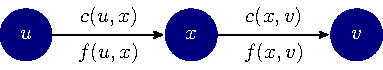
\includegraphics{img/26_1-1/26_1-1_1.pdf}
\end{subfigure}
~
\begin{subfigure}[t]{.45\textwidth}
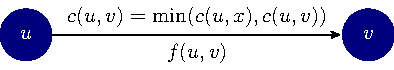
\includegraphics{img/26_1-1/26_1-1_2.pdf}
\end{subfigure}
\caption{Fusionnement d'arête}
\label{fig:edge-fusion}
\end{figure}

Ceci est valide sur un chemin dans lequel tous les sommets intermédiaires $x$ vérifient $d^+(x) = d^-(x) = 1$ (cf. fig. \ref{fig:edge-fusion-2}).


\begin{figure}[H]
\centering
  \begin{subfigure}[t]{\textwidth}
    \centering
    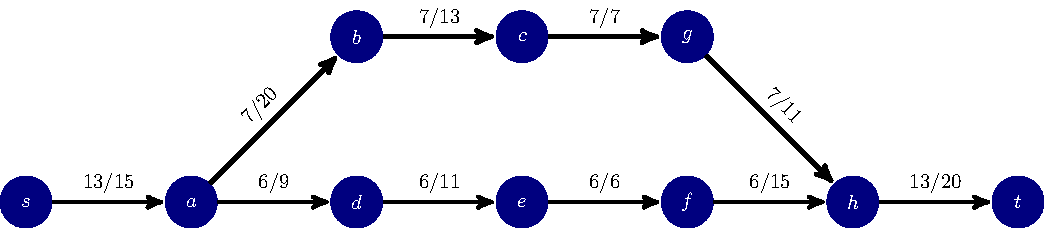
\includegraphics{img/26_1-1/26_1-1_3.pdf}
    \caption{Un réseau $G'$ pouvant être réduit à un réseau équivalent $G$, dans le sens où leur flot maximal sont égaux.}
  \end{subfigure}

  \begin{subfigure}[t]{\textwidth}
    \centering
    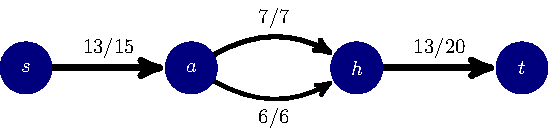
\includegraphics{img/26_1-1/26_1-1_4.pdf}
    \caption{Fusion du chemin $(a,b,c,g,h)$  et du chemin $(a,d,e,f,h)$ en $(a,h)$.}
  \end{subfigure}

  \begin{subfigure}[t]{0.49\textwidth}
    \centering
    
\includegraphics{img/26_1-1/26_1-1_5.pdf}
    \caption{Fusion des deux arêtes $(a,h)$.}
  \end{subfigure}
~
  \begin{subfigure}[t]{0.49\textwidth}
    \centering
    
\includegraphics{img/26_1-1/26_1-1_6.pdf}
    \caption{Le réseau $G$ final.}
  \end{subfigure}
  \caption{Fusionnement de chemin unidirectionnel}
  \label{fig:edge-fusion-2}
  %TODO:TikZ highlight edge instead of add width
\end{figure}
\end{ex}

\descitem{26.1-2} \textit{}
\descitem{26.1-3} \textit{}
\descitem{26.1-4} \textit{}
\descitem{26.1-5} \textit{}
\descitem{26.1-6} \textit{}
\descitem{26.1-7} \textit{}

\end{description}

\section{Multithreaded Algorithms}

\section{Matrix Operations}

\section{Linear Programming}

\section{Polynomials and the FFT}

\section{Number-Theoretic Algorithms}

\section{String Matching}

\subsection{The naive string-matching algorithm}

\begin{description}
\descitem{32.1-1} \textit{Show the comparisons the naive string matcher makes for the pattern $P = 0001
$ in the text $T = 000010001010001$.}

\begin{ex}
    \begin{figure}[H]
      \centering
      \begin{subfigure}[t]{.45\textwidth}
        \centering
        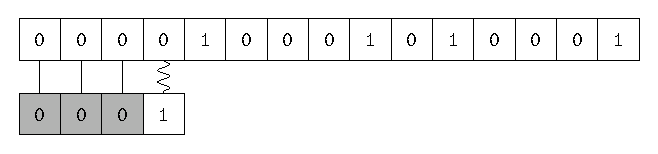
\includegraphics[scale=.6]{img/32_1-1/32_1-1_1.pdf}
        \caption{$\texttt{shift} = 0$}\label{fig:32_1-1_1}
      \end{subfigure}
      \begin{subfigure}[t]{.45\textwidth}
        \centering
        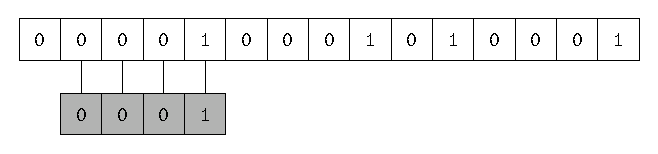
\includegraphics[scale=.6]{img/32_1-1/32_1-1_2.pdf}
        \caption{$\texttt{shift} = 1$}\label{fig:32_1-1_2}
      \end{subfigure}
      \begin{subfigure}[t]{.45\textwidth}
        \centering
        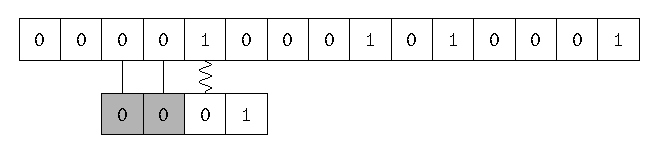
\includegraphics[scale=.6]{img/32_1-1/32_1-1_3.pdf}
        \caption{$\texttt{shift} = 2$}\label{fig:32_1-1_3}
      \end{subfigure}
      \begin{subfigure}[t]{.45\textwidth}
        \centering
        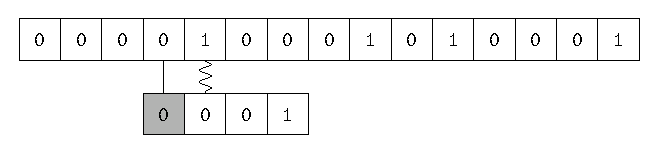
\includegraphics[scale=.6]{img/32_1-1/32_1-1_4.pdf}
        \caption{$\texttt{shift} = 3$}\label{fig:32_1-1_4}
      \end{subfigure}
      \begin{subfigure}[t]{.45\textwidth}
        \centering
        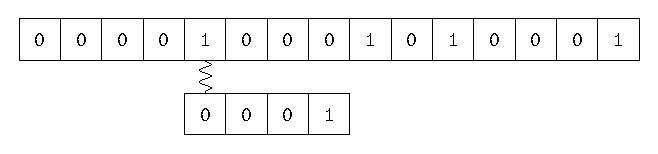
\includegraphics[scale=.6]{img/32_1-1/32_1-1_5.pdf}
        \caption{$\texttt{shift} = 4$}\label{fig:32_1-1_5}
      \end{subfigure}
      \begin{subfigure}[t]{.45\textwidth}
        \centering
        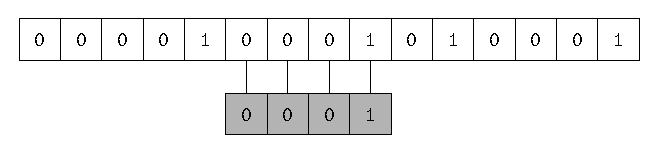
\includegraphics[scale=.6]{img/32_1-1/32_1-1_6.pdf}
        \caption{$\texttt{shift} = 5$}\label{fig:32_1-1_6}
      \end{subfigure}
      \begin{subfigure}[t]{.45\textwidth}
        \centering
        \includegraphics[scale=.6]{img/32_1-1/32_1-1_7.pdf}
        \caption{$\texttt{shift} = 6$}\label{fig:32_1-1_7}
      \end{subfigure}
      \begin{subfigure}[t]{.45\textwidth}
        \centering
        \includegraphics[scale=.6]{img/32_1-1/32_1-1_8.pdf}
        \caption{$\texttt{shift} = 7$}\label{fig:32_1-1_8}
      \end{subfigure}
      \begin{subfigure}[t]{.45\textwidth}
        \centering
        \includegraphics[scale=.6]{img/32_1-1/32_1-1_9.pdf}
        \caption{$\texttt{shift} = 8$}\label{fig:32_1-1_9}
      \end{subfigure}
      \begin{subfigure}[t]{.45\textwidth}
        \centering
        \includegraphics[scale=.6]{img/32_1-1/32_1-1_10.pdf}
        \caption{$\texttt{shift} = 9$}\label{fig:32_1-1_10}
      \end{subfigure}
      \begin{subfigure}[t]{.45\textwidth}
        \centering
        \includegraphics[scale=.6]{img/32_1-1/32_1-1_11.pdf}
        \caption{$\texttt{shift} = 10$}\label{fig:32_1-1_11}
      \end{subfigure}
      \begin{subfigure}[t]{.45\textwidth}
        \centering
        \includegraphics[scale=.6]{img/32_1-1/32_1-1_12.pdf}
        \caption{$\texttt{shift} = 11$}\label{fig:32_1-1_12}
      \end{subfigure}
      \caption{Recherche de la sous châine $0001$ dans $000010001010001$ avec l'algorithme naïve.} 
      \label{fig:naive-match-string} 
    \end{figure}
\end{ex}


\descitem{32.1-2} \textit{Suppose that all characters in the pattern $P$ are different. Show how to accelerate
\proc{Naive-String-Matcher} to run in time $O(n)$ on an $n$-character text $T$.}

\begin{ex}
\begin{codebox}
\Procname{\algo{Naive-String-Matcher-Diff}$(\id{T}, \id{P})$}
    \li $n = \attrib{T}{length}$, $m = \attrib{P}{length}$, $s = 0$
    \li \While $\id{s} \le n -m$ \Do
    \li \If $P[1\twodots m] == T[s + 1\twodots s + m]$ \Then
    \li print "Pattern occurs with shift" s 
    \li $s \gets s + m$ 
    \li \Else 
    \li $s \gets s + 1$ \End
\end{codebox}
\end{ex}

\descitem{32.1-3} \textit{Suppose that pattern $P$ and text $T$ are randomly chosen strings of length $m$ and $n$,
respectively, from the $d$-ary alphabet $\Sigma_d = \{0, 1, \ldots, d-1\}$, where $d \ge 2$. Show
that the expected number of character-to-character comparisons made by the implicit loop in line $4$ of the naive algorithm is
    \[(n-m+1) \frac{1-d^{-m}}{1-d^{-1}} \le 2(n - m + 1)\]
over all executions of this loop. (Assume that the naive algorithm stops comparing
characters for a given shift once it finds a mismatch or matches the entire pattern.)
Thus, for randomly chosen strings, the naive algorithm is quite efficient.  }

\begin{exrev}

\end{exrev}

\descitem{32.1-4} \textit{Suppose we allow the pattern $P$ to contain occurrences of a gap character $\diamondsuit$ that
can match an \textit{arbitrary} string of characters (even one of zero length). For example,
the pattern $ab\diamondsuit ba\diamondsuit c$ occurs in the text $cabccbacbacab$ abstract as}

    $c\smallunderbrace{ab}_{ab}\smallunderbrace{cc}_{\diamondsuit}\smallunderbrace{ba}_{ba}\smallunderbrace{cba}_{\diamondsuit}\smallunderbrace{c}_{c}ab$

\textit{and as}

    $c\smallunderbrace{ab}_{ab}\smallunderbrace{ccbac}_{\diamondsuit}\smallunderbrace{ba}_{ba}\smallunderbrace{}_{\diamondsuit}\smallunderbrace{c}_{c}ab$.

\textit{Note that the gap character may occur an arbitrary number of times in the pattern
but not at all in the text. Give a polynomial-time algorithm to determine whether
such a pattern $P$ occurs in a given text $T$ , and analyze the running time of your
algorithm.}
\begin{ex}

\begin{codebox}
\Procname{\algo{Naive-String-Matcher-With-Gap}$(\id{T}, \id{P}, \id{gap})$}
    \li $n = \attrib{T}{length}$,  $m = \attrib{P}{length}$, $s = 0$
    \li \For each $P_i$ in partition $P$ delimited by $\id{gap}$ character \Do
    \li $m_i = \attrib{P_i}{length}$
    \li \While $s \le n - m_i$ \Do
    \li \If $P_i[1\twodots m_i] == T[s + 1\twodots s + m_i]$ \Then
    \li $\id{shift}[i] \gets s$
    \li \Break \End
    \li $s \gets s + 1$ \End \End
    \li \If $s \le n-m_{\text{last}}$ \Then
    \li print "Pattern occurs with shift" $\id{shift}[1]$ \End
\end{codebox}

Notons $p$ le nombre des patterns $P_i$, $m_{\min}$ et $m_{\max}$ les patterns $P_i$ respectivement plus court et plus long. 
Le \textit{parsing} des $P_i$ nécessite $O(m)$. Puis, en considérant le pseudocode, la recherche de pattern avec trou est en $O(p \cdot (n - m_{\min} + 1) \cdot m_{\max} + m)$. 

Supposons maintenant qu'il n'y a pas de $\diamondsuit$ consécutive dans $P$ et que les sous patterns sont de taille équitable, \textit{i.e.} $\forall i \le p, m_i = \frac{m - p + 1}{p}$. Alors, on a
    \[O(p \cdot (n - m_{\min} + 1) \cdot m_{\max} + m) = O (nm).\]

\end{ex}

\end{description}

\subsection{The Rabin-Karp algorithm}

\begin{description}
\descitem{32.2-1} \textit{Working modulo $q = 11$, how many spurious hits does the Rabin-Karp matcher encounter in the text $T = 3141592653589793$ when looking for the pattern $P = 26$?}
\begin{ex}
Trois, car $26 \equiv 15 \equiv 59 \equiv 92\mod 11$.
\end{ex}
\descitem{32.2-2} \textit{How would you extend the Rabin-Karp method to the problem of searching a text
string for an occurrence of any one of a given set of $k$ patterns? Start by assuming
that all $k$ patterns have the same length. Then generalize your solution to allow the
patterns to have different lengths.}

\begin{ex}
\begin{codebox}
\Procname{\algo{Rabin-Karp-Matcher-$k$-Patterns-Same-Length}$(\id{T}, \id{P}, \id{k}, \id{d}, \id{q})$}
    \li $n = \attrib{T}{length}$,  $m = \attrib{P}{length}$, $h = d^{m-1} \mod q$, $t = 0$
    \li \For $i=0$ \To $k$ \Do
        \li $p[i] = 0$ \End
    \li \For $i=0$ \To $m$ \Comment Preprocessing \Do
      \li \For $j=0$ \To $k$ \Do
        \li $p[j] = (d \cdot p[j] + P[j][i]) \mod q$ \End
      \li $t = (d \cdot t + T[i]) \mod q$ \End
    \li \For $s = 0$ \To $n - m$ \Comment Matching \Do
      \li \For $j=0$ \To $k$ \Do
        \li \If $p[j] == t$ \Then
           \li \If $P[j][1 \twodots m] == T[s + 1 \twodots s + m]$ \Then
             \li print "Pattern" $P[j]$ "occurs with shift" $s$ 
           \End
        \End
      \End
      \li \If $s < n - m$ \Then
        \li $t = (d \cdot (t - T[s+1] \cdot h) + T[s + m + 1]) \mod q$
      \End
   \End
\end{codebox}
\begin{codebox}
\Procname{\algo{Rabin-Karp-Matcher-With-$k$-Patterns-Diff-Length}$(\id{T}, \id{P}, \id{k}, \id{d}, \id{q})$}
    \li $n = \attrib{T}{length}$
    \li \For $i=0$ \To $k$ \Do
        \li $p[i] = 0$ 
        \li $t[i] = 0$ 
        \li $m_i = \attrib{P[i]}{length}$
        \li $h[i] = d^{m_i - 1} \mod q$ 
    \End
    \li \For $i=0$ \To $m_{\max}$ \Comment Preprocessing \Do
      \li \For $j=0$ \To $k$ \Do
        \li \If $i < m_j$ \Then 
          \li $p[j] = (d \cdot p[j] + P[j][i]) \mod q$ 
          \li $t[j] = (d \cdot t[j] + T[i]) \mod q$ 
        \End
      \End
    \End
    \li \For $s = 0$ \To $n - m_{\min}$ \Comment Matching \Do
      \li \For $j=0$ \To $k$ \Do
        \li \If $p[j] == t$ \Then
           \li \If $P[j][1 \twodots m_j] == T[s + 1 \twodots s + m_j]$ \Then
             \li print "Pattern" $P[j]$ "occurs with shift" $s$ 
           \End
        \End
      \End
      \li \If $s < n - m_{\min}$ \Then
        \li \For $i=0$ \To $k$ \Do
          \li $t[i] = (d \cdot (t[i] - T[s+1] \cdot h[i]) + T[s + m[i] + 1]) \mod q$
        \End
      \End
   \End
\end{codebox}
\end{ex}

\descitem{32.2-3} \textit{}
\descitem{32.2-4} \textit{}
\end{description}


\section{Computational Geometry}

\section{NP-Completeness}

\section{Approximation Algorithms}


\appendix
\clearpage
\part{Appendix: Mathematical Background}
\section{Summation}

R\'ef\'erences : \cite{uic_hw1}

\subsection{Summation formulas and propreties}

\begin{description}
  \item [A.1-1] {\itshape Find a simple formula for $\sum_{k=1}^n(2k-1)$ }
   \begin{ex}
  \begin{align*}
    \sum_{k=1}^n(2k-1)  & = n(n+1)-n\\
    &= n^2.
  \end{align*}
\end{ex}
\item[A.1-2 $\star$]  {\itshape Show that $\sum_{k=1}^n1/(2k-1) = \ln (\sqrt{n}) + \O(1)$ by manipulating the harmonic series.}
    \begin{ex}
      \begin{align*}
        \sum_{k=1}^n \frac{1}{2k-1} &= H_n - \frac{1}{2}\sum_{k=1}^n\frac{1}{k}\\
       &= \frac{1}{2}H_n\\
       &= \ln(\sqrt{n}) + \O(1).
      \end{align*}
    \end{ex}
  \item[A.1-3] {\itshape Show that $\sum_{k=0}^{\infty} k^2x^k = x(1+x)/(1-x)^3$ for $ 0 < |x| < 1$.}
    \begin{ex}
    \begin{align*}
  \sum_{k=0}^\infty k^2x^k & = x \left( \frac{x}{(1-x)^2} \right)^\prime\\
      &= \frac{x}{(1-x)^2}+\frac{2x}{(1-x)^3}\\
      &= \frac{x(1+x)}{(1-x)^3}.
    \end{align*}
  \end{ex}
\item[A.1-4 $\star$] {\itshape Show that $\sum^\infty_{k=0}(k-1)/2^k = 0$.}
    \begin{ex}
    Soit $S=\sum_{k=0}^\infty\frac{k-1}{2^k}$. Alors $2S = \sum_{k=0}^{\infty}\frac{k-1}{2^{k-1}}= -2 + \sum_{k=0}^\infty\frac{k}{2^k}$. Donc 
    \begin{align*}
      2S-S &= -2 + \sum_{k=0}^\infty\frac{1}{2^k}\\
      &= 0.
     \end{align*}
   \end{ex}
 \item[A.1-5 $\star$] {\itshape Evaluate the sum $\sum_{k=1}^\infty(2k+1)x^{2k}$ for $|x| < 1$.}
   \begin{ex}
    \begin{align*}
      \sum_{k=1}^{\infty}(2k+1)x^{2k} &= \left(\sum_{k=1}^\infty x^{2k+1}\right)^\prime\\
    &= \left(\frac{x}{1-x^2} - x\right)^\prime\\
      &= \frac{3x^2}{1-x^2} + \frac{2x^4}{(1-x^2)^2}
    \end{align*}
  \end{ex}
  \item[A.1-6] {\itshape  Prove that $\sum_{k=1}^n\O(f_k(i)) = O\left(\sum_{k=1}^n f_k(i)\right)$ by using the linearity proprety of summations.}
    \begin{ex}
    Soit pour tout $k \in \llbracket 1, n \rrbracket, g_k \in \O(f_k)$, autrement dit $g_k \le c_kf_k$ est v\'erifi\'e \`a partir d'un rang $N_k$ avec $c_k > 0$. On a donc $\sum_{k=1}^n g_k \le \sum_{k=1}^ncf_k$ v\'erifi\'e \`a partir d'un rang $N = \max(N_1, \ldots,N_n)$ et $c = \max(c_1, \ldots,c_n)$ . D'o\`u $\sum_{k=1}^n g_k \in \O(\sum_{k=1}^n f_k)$.
  \end{ex}
\item[A.1-7] {\itshape Evaluate the product $\prod_{k=1}^n2\cdot 4^k$.}
    \begin{ex}
  Soit $P=\prod_{k=1}^n2\cdot4^k = \prod_{k=1}^n2^{2k+1}$. On a 
  \begin{align*}
    \lg P &= \sum_{k=1}^n2k+1\\
    &= n(n+2)
  \end{align*}

  Finalement, $P = 2^{n(n+2)}$.
    \end{ex}
  \item[A.1-8 $\star$] {\itshape Evaluate the product $\prod_{k=2}^n(1-1/k^2)$.}
    \begin{ex}
  \begin{align*}
    \prod_{k=2}^n(1-\frac{1}{k^2}) &= \prod_{k=2}^n \frac{k-1}{k}\cdot\frac{k+1}{k}\\
      &= \frac{1}{2}\cdot\frac{n+1}{n}\\
      &= \frac{n+1}{2n}.
  \end{align*}
    \end{ex}
\end{description}

  \subsection{Bounding summations}

  \begin{description}
    \item[A.2-1] {\itshape Show that $\sum_{k=1}^n 1/k^2$ is bounded above by a constant.}
      \begin{ex}
      \begin{align*}
        \sum_{k=1}^n\frac{1}{k^2} &= 1 + \sum_{k=2}^n\frac{1}{k^2}\\
        &\le 1 + \int_1^n\frac{1}{x^2}\diff x\\
        &= 1 + (1-\frac{1}{n})\\
        &= 2 - \frac{1}{n}\\
        &\le 2.
      \end{align*}
    \end{ex}
    \item[A.2-2]{\itshape Find an asymptotic upper bound on the summation $\sum\limits_{k=0}^{\lfloor \lg n \rfloor}\lceil n/2^k \rceil$.}

    \item[A.2-3] {\itshape Show that the $n$th harmonic number is $\Omega(\lg n)$ by splitting the summation.}

    \item[A.2-4]{\itshape Approximate $\sum_{k=1}^nk^3$ with an integral.}
        \begin{ex}
      On a
      $$\int_0^nx^3\diff x \le \sum_{k=1}^nk^3 \le \int_1^{n+1}x^3\diff x$$ ce qui donne $$\frac{n^4}{4} \le \sum_{k=1}^nk^3 \le \frac{(n+1)^4-1}{4}.$$ Ainsi, $\sum_{k=1}^nk^3 = \Theta(n^4)$.
    \end{ex}

  \item[A.2-5] {\itshape Why didn’t we use the integral approximation (A.12) directly on $\sum_{k=1}^n1/k$ to obtain an upper bound on the {\itshape n}th harmonic number?}
    \begin{ex}
      Car la primitive de $1/x$ n'est pas d\'efinie en $0$.
    \end{ex}

  \end{description}

  \subsection{Problems}

  \begin{description}
    \item[A-1] {\itshape \bfseries Bounding summations}

        {\itshape Give asymptotically tight bounds on the following summations. Assume that $r > 0$ and $s > 0$ are constants.}

        \begin{Al}
          \item $\sum\limits_{k=1}^nk^r$.
          \item $\sum\limits_{k=1}^n\lg^sk$.
          \item $\sum\limits_{k=1}^nk^r\lg^sk$
        \end{Al}

        \begin{pbrev}
        \end{pbrev}

  \end{description}

\section{Sets, Etc.}

\section{Counting and Probability}

\subsection{Counting}

\begin{description}
  \item[C.1-1] {\itshape How many $k$-substrings does an $n$-string have? (Consider identical $k$-substrings at different positions to be different.) How many substrings does an $n$-string have in total?}
    \begin{ex}
      Il y a $S_k = n - k + 1$ $k$-sous-cha\^ines dans une $n$-cha\^ine. Le nombre total de sous-cha\^ines dans une $n$-cha\^ine est donc \[\sum_{k=1}^n S_k = \frac{n(n+1)}{2}.\]
    \end{ex}
  \item[C.1-2] {\itshape An $n$-input, $m$-output boolean function is a function from  $\{\textrm{TRUE}, \textrm{FALSE}\}^n$ to $\{\textrm{TRUE}, \textrm{FALSE}\}^m$. How many $n$-input, $1$-output boolean functions are there? How many $n$-input, $m$-output boolean functions are there?}
    \begin{ex}
      Le cardinal de l'ensemble de fonction de $E$ dans $F$  est $|F|^{|E|}$. Particuli\`erement pour les fonctions bool\'eenes, on a :
      \begin{itemize}
        \item pour $E = \{\textrm{TRUE}, \textrm{FALSE}\}^n$ et $F=\{\textrm{TRUE}, \textrm{FALSE}\}$, $|F|^{|E|} = 2^{2^n}$ ;
        \item pour $E = \{\textrm{TRUE}, \textrm{FALSE}\}^n$ et $F=\{\textrm{TRUE}, \textrm{FALSE}\}^m$, $|F|^{|E|} = {(2^m)}^{2^n}$.
      \end{itemize}
    \end{ex}
  \item[C.1-3] {\itshape In how many ways can $n$ professors sit around a circular conference table? Consider two seatings to be the same if one can be rotated to form the other.}

    \begin{ex}
      On consid\`ere tout d'abord le cas de si\`eges rang\'es lin\'eairement. Dans ce cas, on a $n!$ arrangements. Dans le cas circulaire, on peut d\'efinir une relation d'\'equivalence $\mathcal{R}$ qui regroupe les arrangements qui peuvent \^etre obtenus par une permutation circulaire. De ce fait, il y a exactement $n$ \'el\'ements dans chaque classe. Le nombre d'arrangement de si\`eges plac\'es circulairement est en fait le cardinal de l'espace quotient\'e par $\mathcal{R}$. Donc il y a $\frac{n!}{n} = (n-1)!$ arrangements.
    \end{ex}

  \item[C.1-4] {\itshape In how many ways can we choose three distinct numbers from the set $\{1, 2,\ldots, 99\}$ so that their sum is even?}
    \begin{ex}
      Pour obtenir un nombre pair en sommant trois nombres distincts de l'ensemble $E = \{1, 2, \ldots, 99\}$, il y a deux possibilit\'es :
      \begin{itemize}
        \item pair + pair + pair = pair ;
        \item impair + impair + pair = pair .
      \end{itemize}
      Dans l'ensemble $E$, il y a $50$ nombres impairs et $49$ nombres pairs. Finalement, le nombre de combinaisons est :
      \[ \binom{49}{3} + \binom{50}{2}\binom{49}{1} = 78449.  \]
      
    \end{ex}
  \item[C.1-5] {\itshape Prove the identity \[\binom{n}{k} = \frac{n}{k}\binom{n-1}{k-1}\] for $ 0 < k \le n$.}

    \begin{ex}
      \[ \binom{n}{k} = \frac{n!}{k!(n-k)!} = \frac{n\cdot(n-1)!}{k(k-1)!((n-1)-(k-1))!} = \frac{n}{k}\binom{n-1}{k-1}.\]
    \end{ex}

  \item[C.1-6] {\itshape Prove the identity \[\binom{n}{k} = \frac{n}{n-k}\binom{n-1}{k}\] for $ 0 \le k < n$.}
    \begin{ex}
      \[ \binom{n}{k} = \frac{n}{n-k}\cdot\frac{(n-1)!}{k!((n-1)-k)!} = \binom{n-1}{k}.\]
    \end{ex}
  \item[C.1-7] {\itshape To choose $k$ objects from $n$, you can make one of the objects distinguished and consider whether the distinguished object is chosen. Use this approach to prove that \[\binom{n}{k} = \binom{n-1}{k}+\binom{n-1}{k-1}.\]}
    \begin{ex}\mbox{}\\ %TODO: fix diagram
      {
        \begin{figure}[H]
          \centering
        \includegraphics[scale=1.5]{img/C_1-7/C_1-7.pdf}
        \caption{\frquote{combinaison de $k$ parmi $n$}}
          \label{fig:C.1-7}
        \end{figure}
      }
      On fixe un \'el\'ement parmi les $n$ et on en choisit $k$. Si l'\'el\'ement est choisi, il y a $\binom{n-1}{k-1}$ moyens de choisir les autres; sinon les $k$ \'el\'ements choisis sont inclus dans les $n-1$ restants et il y a $\binom{n-1}{k}$ moyens de choisir.
    Conclusion : $ \binom{n}{k} = \binom{n-1}{k}+\binom{n-1}{k-1}$, d'o\`u ce que montre la figure (\ref{fig:C.1-7}).     
    \end{ex}
  \item[C.1-8] {\itshape Using the result of Exercise C.1-7, make a table for $n = 0, 1, \ldots, 6$ and $ 0\le k \le n$ of the binomial coefficients $\binom{n}{k}$ with $\binom{0}{0}$ at the top, $\binom{1}{0}$ and $\binom{1}{1}$ on the next line, and so forth. Such a table of binomial coefficients is called \textbf{Pascal’s triangle}.}
    \begin{ex}\mbox{}
      \begin{figure}[H]
        \centering
        \includegraphics{img/C_1-8/C_1-8.pdf}
        \caption{Triangle dit de Yang Hui ou de Pascal}
        \label{fig:}
      \end{figure}
    \end{ex}
  \item[C.1-9] {\itshape Prove that \[ \sum_{i=1}^n i = \binom{n+1}{2}.\]}
    \begin{ex}
      \[\sum_{i=1}^ni = \frac{n(n+1)}{2} = \frac{(n+1)!}{(n-2)!2!} = \binom{n+1}{2}.\]
    \end{ex}
  \item[C.1-10] {\itshape }
  \item[C.1-11 $\star$] {\itshape }
  \item[C.1-12 $\star$] {\itshape }
  \item[C.1-13 $\star$] {\itshape }
  \item[C.1-14 $\star$] {\itshape }
  \item[C.1-15 $\star$] {\itshape }
\end{description}

\section{Matrices}

\subsection{Matrices and matrix operations}

\begin{description}
  \descitem{D.1-1} \textit{Show that if $A$ and $B$ are symmetric $n \times n$ matrices, then so are $A + B$ and $A - B$.}
    \begin{ex}
        Il est clair que $A \pm B = A^\T \pm B^\T = (A \pm B)^\T$.
    \end{ex}
  \descitem{D.1-2} \textit{Prove that $(AB)^\T$ and that $A^\T A$ is always a symmetric matrix.}
    \begin{ex}
    Supposons que $A$ et $B$ sont respectivement de type $(n, m)$ et $(m,p)$. On a Alors
        \begin{align*}
          (AB)^\T_{ij} &= \left( \sum_{k=1}^m a_{jk}b_{ki} \right)_{\substack{i\le p\\j\le n}}\\
          &=\left( \sum_{k=1}^m \hat{b}_{ik}\hat{a}_{kj} \right)_{\substack{i\le p\\j\le n}}\\
          &= B^\T A^\T
        \end{align*}
    où $B^\T = (\hat{b}_{ij})$ et $A^\T = (\hat{a}_{ij})$. Ainsi $(A^\T A)^\T = A^\T A$, donc $A^\T A$ est symétrique.

    On peut aussi voir la matrice $A_{nm}$ comme $m$ vecteurs colonne $(a_i)_{i\le m}$ concaténés. Le produit $C := A^\T A$ n'est rien d'autre que le produit scalaire : $\forall i, j \in \llbracket 1, n \rrbracket, c_{ij} = \langle a_i, a_j \rangle$. Le produit scalaire est une forme bilinéaire définie positif \textit{symétrique}.
    \end{ex}
  \descitem{D.1-3} \textit{Prove that the product of two lower-triangular matrices is lower-triangular.}
  \begin{ex}
    Soit $A, B$ deux matrices triangulaires inférieurs et posons $C = AB$. Montrons que pour tout $i < j$, $c_{ij} = 0$ :
        \begin{align*}
          c_{ij} &= \sum_{k=1}^n a_{ik}b_{kj}\\
          &= \sum_{k=1}^{j-1} a_{ik}b_{kj} + \sum_{k=j}^{n} a_{ik}b_{kj}\\
          &= 0.
        \end{align*}
  \end{ex}
  \descitem{D.1-4} \textit{}
\end{description}

\subsection{Basic matrix propreties}


% \setglossarystyle{mylist}

%  \clearpage
%  \phantomsection
%  \addcontentsline{toc}{section}{Acronymes}
%  \printglossary[type=\acronymtype]

% \clearpage
% \phantomsection
% \addcontentsline{toc}{section}{Glossaire}
% \printglossary[type=main]

% \clearpage
% \phantomsection
% \addcontentsline{toc}{section}{Index}
% \printindex

\clearpage
\phantomsection
\addcontentsline{toc}{section}{Références}
\bibliographystyle{plain}
\bibliography{main.bib}
\nocite{*}

\end{document}
